% vim:ft=tex
\documentclass[a4paper,11pt]{scrartcl}
\usepackage{tohojo-xe}
%\selectlanguage{english}
\setcounter{secnumdepth}{3}
\setcounter{tocdepth}{2}
\hypersetup{pdfauthor={Toke Høiland-Jørgensen, Mikkel Hartmann, Dan 
Albrechtsen, Malik Thrane, Troels Christensen, Wence Xiao}, pdftitle={Crowd 
modelling}}

\title{Crowd modelling}
\author{Toke Høiland-Jørgensen, Mikkel Hartmann, Dan Albrechtsen, Malik 
Thrane, Troels Christensen, Wence Xiao}
\date{2010-09-12}
\fancyhead[OR,EL]{\footnotesize Draft: \timestamp}
%\type{}
\begin{document}

\begin{titlepage}
    \begin{center}
        {\Huge \sffamily \textbf{Crowd modelling\\[2cm]
        }}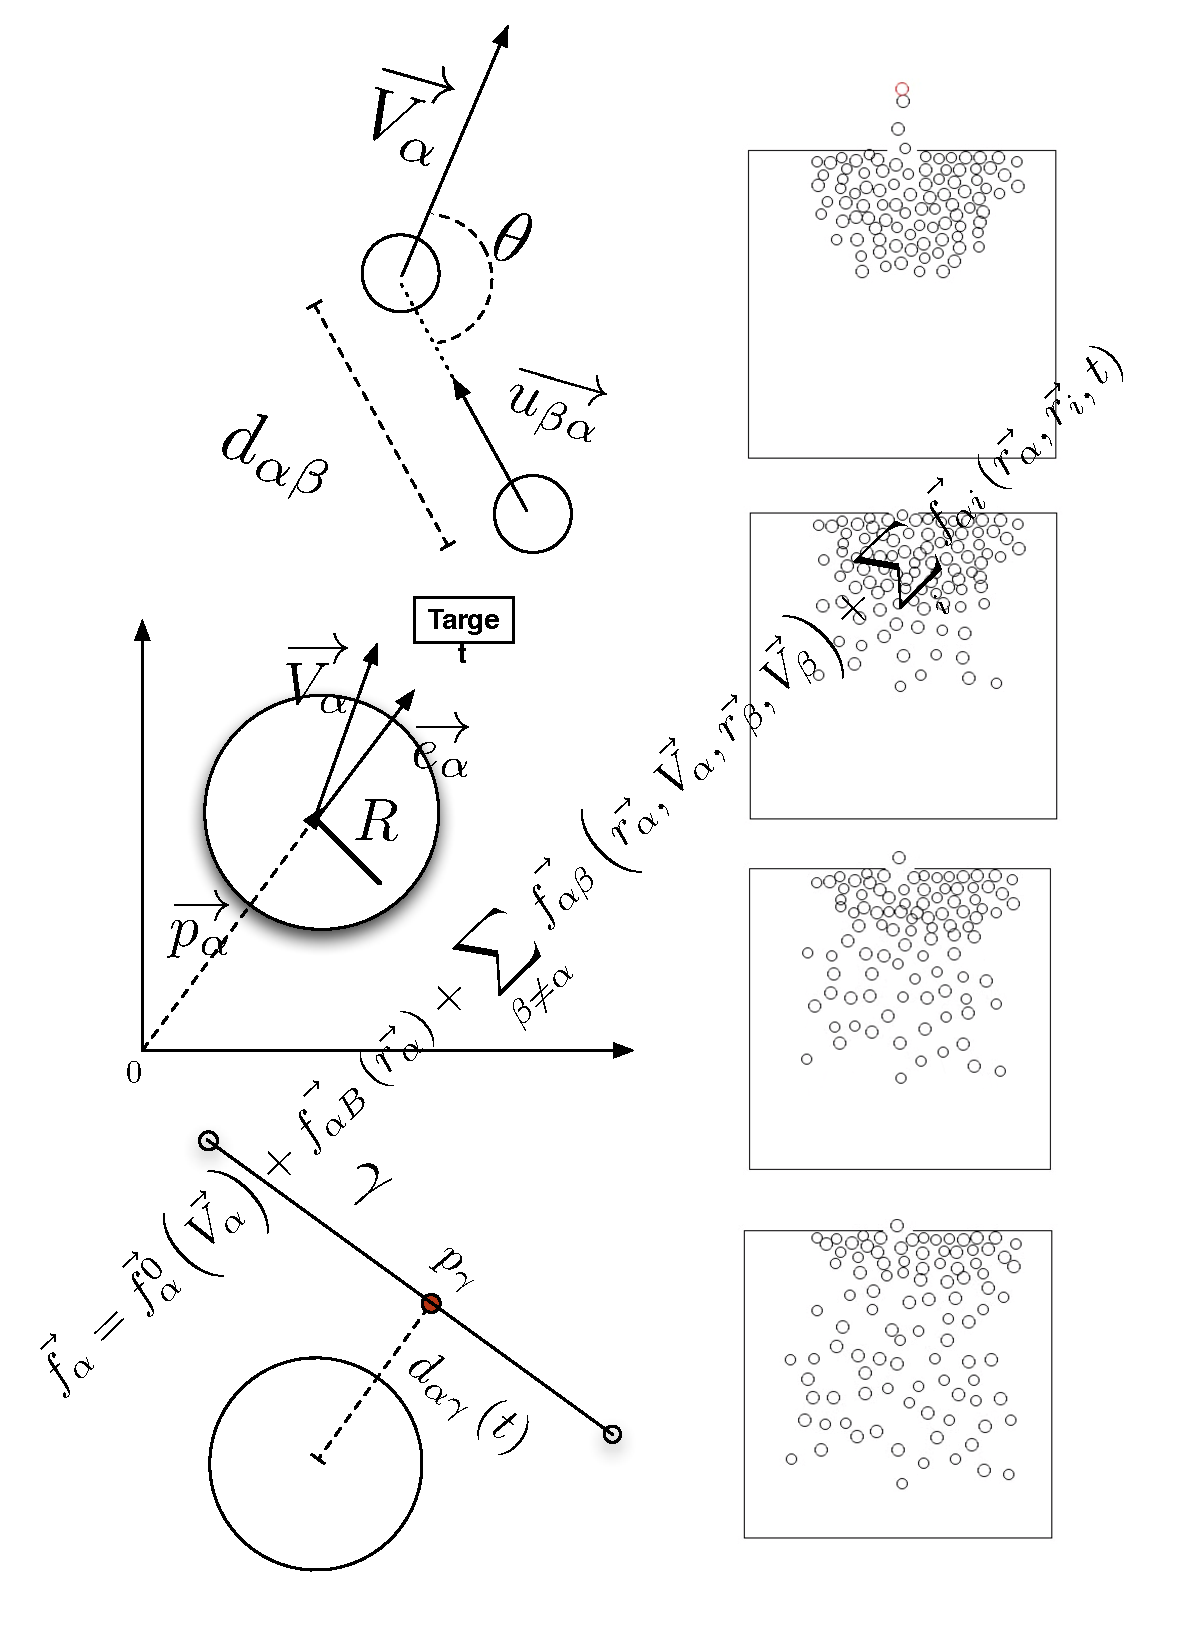
\includegraphics[width=10cm]{Figures/Frontpage}
        \\[2cm]

        {\large Toke Høiland-Jørgensen \\
        Mikkel Hartmann\\
        Dan Albrechtsen\\
        Malik Thrane\\
        Troels Christensen\\
        Wence Xiao\\
        [0.5cm] }

        {\small \textbf{\textsf{Advisor}}\\
        Viggo Andreasen}
        \vfill
        \textsf{Modelling project, fall 2010\\
        Mathematics RUC}
	\end{center}

    \clearpage
%    % vim:ft=tex

\begin{abstract}
    \section*{Abstract}
    \small
    We look at social force models as a way to model the behaviour of human 
    crowds, in order to evaluate what these types of models can tell us about 
    crowds, which assumptions underlie them and what their strengths and 
    weaknesses are. In order to do this evaluation, we implement a computer 
    simulation of an exemplary social force model.

    In order to create this simulation, we pick an exemplary model that is 
    described in detail in the article that presents it, and analyse it in 
    detail, filling in details from other articles where necessary. Based on 
    this analysis of the model, we go from the abstract model formulation to a 
    concrete numerical simulation by filling in required details, such as  how 
    to approximate the movement of pedestrians, how to set initial conditions 
    and values, and how to implement the interaction between pedestrians and 
    walls in practice.

    From our results, it is clear that our simulation (with the right 
    parameters) exhibits reasonable pedestrian behaviour upon visual 
    inspection. While we successfully replicate some results from the 
    literature, other effects do not manifest themselves. We discuss several 
    reasons for this discrepancy, including features that are lagging from the 
    model, parameter values, effects of using random numbers to generate the 
    initial conditions and possible errors in our implementation of the model.

    Based on the results of our own simulations and our review of the social 
    force modelling field, we assess social force models and their strengths 
    and weaknesses. We conclude that social force models are not built on any 
    theories for the behaviour of crowds, but are created to replicate a set 
    of observations. As such, any confidence in their predictions must come 
    from a record of producing results fitting observations; and since the 
    field is relatively new, they have not yet reached this state. Social 
    force models do, however, provide a practical way to simulate something 
    that would otherwise be impossible to simulate. As such, they are the best 
    available way to provide e.g. guidance when designing facilities that must 
    accommodate many pedestrians, and given time the accuracy of their 
    predictions will probably increase.
\end{abstract}
\begin{abstract}
    \section*{Resume}
    \small
\end{abstract}

\end{titlepage}

\tableofcontents
\listoffigures

\clearpage

% vim:ft=tex
\section{Introduction}
When a lot of people are gathered in a confined space, it is not immediately 
obvious how they behave when moving around. It is also not obvious how to 
design buildings and other areas where many people gather to allow for optimal 
passage of crowds without jamming and related problems (such as inconvenience 
for pedestrians and even injuries). It is cumbersome, or even dangerous, to 
gather many people together to do experiments, especially if one wishes to 
simulate a panic situation (which cannot necessarily be induced artificially).  
It would thus be useful to be able to model a crowd of pedestrians and their 
movement.

A crowd of many people is a very complex system. One of the approaches to 
handling this complexity is by using a computer simulation of a model derived 
from the behaviour of individual pedestrians, and through the outcome of this 
simulation be able to say something meaningful about the whole system. This 
approach to modelling complex systems is called agent-based modelling and is 
used in many different and diverse subject areas, including molecular biology, 
economics and physics.

Within the field of crowd simulations, there  are various ways of formulating 
such an agent-based model; we have chosen to focus on an approach that models 
pedestrian behaviour using a concept called ``social forces'' 
\cite{social-force}. This type of model describes individual behaviour 
borrowing concepts and notation from physics, by defining  virtual ``forces'' 
representing desired movement as well as the tendency to avoid obstacles, 
other people etc. Through computer simulations this can be used to say 
something about the whole system of moving pedestrians.

Since the original formulation of the social force concept, it has been 
revised several times (e.g.  \cite{helbing00}). For this project we base our 
analysis on the  version presented in \cite{self-org}, as this article goes 
into a reasonable level of detail. We will, however, also include other 
variants where necessary.  Our chosen model, and others like it, describe a 
set of properties of crowd behaviour that has been seen in observations of 
actual crowds as well as replicated in computer simulations.  We think it will 
be interesting to go into detail with this type of model and look into how 
they work and what they can tell us about crowds. This brings us to our 
problem formulation:

\subsection{Problem formulation}
\begin{quote}
    How do social force models work and what do they say about crowds?

    What are the assumptions underlying social force models, and what are 
    their strengths and limitations?
\end{quote}

Our problem is exemplary to mathematical modelling for several reasons. First 
of all, it is an example of applying mathematical theory to a field outside of 
mathematics itself. The field we are working with (crowd simulation) is 
relatively new, but has some established research\footnote{See the overview of 
the field in section~\ref{sec:social-forces}.}. The model itself contains a 
non-trivial application of mathematics and is an example of a type of model 
(agent-based models) used in many cases to study a complex system of 
interacting pedestrians by describing the individual behaviour of the pedestrians and 
using simulations to derive meaningful properties for the whole system. These 
factors combined makes our problem exemplary.
% TODO: References for agent-based models.

\subsection{Target audience}
The target audience of this report is comprised of students of mathematics on 
a level of education similar to our own. This means that we consider 
mathematical concepts and theory that is covered in the bachelor courses at 
the mathematics department at RUC as known subject matter, and will therefore 
not explain these concepts in detail. Concepts that are beyond this are 
explained as necessary. In the description of the simulation program code, 
some familiarity with basic constructs of computer programming is assumed, and 
are thus not explained.

\subsection{Approach to answering the problem formulation}
To answer the problem formulation, it is first necessary to establish the 
concept of social force models in more detail, as well as give an overview 
over the work in the field. This is presented in 
section~\ref{sec:social-forces}, where we also present the model we have chosen 
to focus on, including the results presented in it.

In order to better understand the model, we are going to make our own computer 
simulation of it. To do so, we will first describe the model thoroughly. In 
section~\ref{sec:the-model}, we will go over the different parts and 
parameters of the model, and point out parts that are ambiguous or missing 
from the article presenting the model.  Based on this description, we will 
discuss what is needed to turn the model into a numerical simulation, and how 
we have done so, in section~\ref{sec:model-to-simulation}.

Based on our analysis of the model, we will construct a computer simulation of 
it, modelling cases analogous to those presented in 
section~\ref{sec:social-forces}. Our implementation of the 
simulation is discussed in section~\ref{sec:simulation}, including set up of 
parameters and initial conditions, the structure of our simulation and how we 
obtain results from it.

The actual results of the simulation is addressed in 
section~\ref{sec:results}. Here we present the outcome of our simulation, and 
whether or not we have been able to replicate the results we were aiming for.  
Based on this presentation, we discuss in section~\ref{sec:discussion} 
possible reasons for any discrepancies between our own results and the results 
we are trying to replicate, as well as which alterations of the model would 
be needed to fix them.

Based on our results and the proposed changes to the model, we will assess 
social force models in general in section~\ref{sec:assessment}, giving an 
overview of the strengths and weaknesses of this modelling approach. Finally, 
we will give a summary of our findings and an overview of the whole project in 
section~\ref{sec:conclusion}.

\clearpage
\section{Social force models}
\label{sec:social-forces}
One would think that the motion and dynamics of a human crowd would be
governed by complex human decision making. However, the idea of social force
models is modelling the behaviour using only a set of simple forces to
describe the behaviour of the human pedestrians that comprise a crowd 
\cite{social-force}.

This works by calculating a set of social forces affecting each pedestrian in 
the system.  These forces are not real physical forces but rather a measure of 
the  pedestrians' motivation for acting in specific ways. However the name 
\emph{social forces} is not accidental: both notation and to some extent the 
interpretation is borrowed from physics.

Borrowing the concept of forces from physics  means that pedestrian movement 
is calculated from the social forces using established methods from physics, 
i.e. equations of motion. This means that forces can be summed to generate a 
resulting force for a pedestrian, and that this resulting force can be used to 
describe an acceleration, and thus affect the movement of the pedestrian.

However, social forces differ from physical forces in key areas. Social forces 
are a way to estimate a pedestrian's behaviour and tendency to move in a 
certain direction. As such they do not deal with the physical effects of the 
environment the pedestrian is in, but rather the pedestrian's perception of 
this environment. For example, pedestrians' attempt to avoid colliding with 
each other, which is modelled as a repulsive force between them. This means 
that the forces are not bound by the laws of physics; they can affect 
pedestrians over a distance, whereas a physical force between two pedestrians 
only occur when they are touching. Also, the forces do not obey Newton's third 
law of motion, since they do not represent an actual interaction between 
pedestrians, but only a desire to move in a certain direction. Finally, it 
does not make sense to talk about the results of the forces in terms of 
physical forces. This means that it does not make sense to talk about, e.g., 
pressure by measuring the magnitude of the forces a pedestrian is subjected 
to.

Throughout the report, whenever we refer to forces we mean social forces, 
unless stated otherwise. In the following we give an overview of which 
variants of social force models exist and how they differ, and of the results 
that have been obtained from simulations using these models.

\subsection{Variants of social force models}
Social force models can be found in several variants in the literature. The 
basic idea is the same in all of these variants, but some details differ, such 
as the exact forces included in the models; sometimes even in contradictory 
ways. In this section we outline the different variants of social force 
models. As mentioned in the introduction, we base our analysis and simulations 
on the variant presented in \cite{self-org}. Therefore, the review presented 
here will use this variant as a basis for comparisons.

The model we are using considers all pedestrians to be circular with a given 
radius. This is obviously a simplification, and indeed one of the advances in 
later versions of social force models, is introducing elliptically shaped 
pedestrians, which is seen to yield results that better match experiments made 
in real life \cite{ABconstant}.

Another modification that is seen in other articles is the adding of 
additional forces, such as velocity-dependent repulsive forces, or forces that 
are perpendicular to the direction of the repulsion 
\cite{helbing00,ABconstant}. The latter may be used 
both as a means of simulating a tendency of pedestrians to avoid each other, 
and as a frictional force when pedestrians touch.

Finally, there are models that add an additional layer on top of the social 
force models, to simulate higher-level decisions such as path finding and 
communication between pedestrians as well as incorporating pedestrians that 
get hurt in dense crowds and fall down and turn into obstacles \cite{HiDAC}.


The different variations do not really make a difference when looking at the 
results, according to \cite{self-org}:

\begin{quote}
    One may, of course, take into account other details such as a velocity 
    dependence of the forces and non circular shaped pedestrian bodies, but 
    this does not have qualitative effects on the dynamical phenomena 
    resulting in the simulations. In fact, most observed self-organization 
    phenomena are quite insensitive to the specification of the interaction 
    forces, while it may, of course, influence the quantitative results.
\end{quote}

However, in our simulations we have been unable to replicate several of the 
results presented elsewhere, which contradicts the above quote. This is 
discussed further in sections~\ref{sec:results} and \ref{sec:discussion}.


\subsection{Results obtained from the models}
\label{sec:article-results}
To have something to compare our own simulation results with, we are going to 
attempt to replicate some of the results obtained from other social force 
model simulations. In this section we present the different results and their 
sources. We also list the scenarios we are going to simulate to replicate the 
results.

There are four main results we are going to attempt to replicate: lane 
formation, the ``freezing-by-heating effect'', oscillatory flows at 
bottlenecks and the ``faster-is-slower effect''.

\begin{itemize}
    \item \textbf{The ``faster-is-slower effect''.}  This effect appears when 
        a crowd of pedestrians try to exit through a narrow passageway, such 
        as a door leading out from a room. It has been observed that when 
        pedestrians attempt to move faster (e.g. in panic situations) it will 
        actually result in a \emph{longer} time for all pedestrians to leave 
        the room, because pedestrians block each other on the way out 
        \cite{helbing00}. This effect can also occur when pedestrians are 
        walking along a passageway that widens and then narrows again; faster 
        pedestrians will try to overtake the slower, causing a jam when the 
        passageway narrows \cite{self-org}.

    \item \textbf{Lane Formation} occurs when pedestrians are walking towards 
        each other from opposite directions. The effect is caused by 
        pedestrians walking in the same direction lining up behind each other 
        and walking behind each other in lanes. This effect is seen in 
        simulations as well as in observations of real-life crowd behaviour 
        and is obvious when viewing drawings of the simulation 
        \cite{self-org}.
        
    \item \textbf{The ``freezing-by-heating effect''.} This phenomenon also 
        occurs when pedestrians are walking towards each other from opposite 
        directions. The effect is seen as a clogging up of the passageway when 
        pedestrians try to move past each other. When exhibiting this effect, 
        the clogging is more pronounced when pedestrian velocities increase, 
        which gives rise to the name, that refers to the states of physical 
        matter. Normally higher energy (faster movement of particles) in 
        matter increases the entropy of the matter, (i.e.  heating a liquid 
        turns it into gas), but in this case (when viewing pedestrians as 
        particles and the crowd as matter) the opposite is seen: increasing 
        the energy (velocity) makes pedestrians stand still, corresponding to 
        freezing of matter \cite{frebyheat}.
        
    \item \textbf{Oscillatory Flows at Bottlenecks.}
        This effect arises when pedestrians are moving in opposite directions 
        and pass through a bottleneck, i.e. a narrowing of the passageway.  
        When it is not possible for groups of pedestrians to pass each other 
        at the bottleneck, crowds will line up on both sides of the 
        bottleneck, trying to push through.This results in an oscillatory flow 
        when small groups of pedestrians will pass through in one direction, 
        making room for a small group to pass through in the other, and so on.
        This can be seen as oscillations in the measured flow rate in each 
        direction and has been seen in both simulations and real life 
        observations \cite{self-org}.
\end{itemize}

\subsection{Simulation scenarios}
To attempt to replicate the results presented in the preceding section, we 
will simulate two main scenarios: a square room and a corridor, with a few 
variations.

To try to replicate the faster-is-slower effect, we will simulate 
a square room filled with pedestrians, that all try to exit through the same 
exit. To replicate the other effects, we will simulate a corridor in several 
variations. In the simple case, we will simulate a plain corridor with 
pedestrians walking in both directions, and see if we get lane formation and 
freezing by heating. We will simulate a corridor with a narrowing in the 
middle to simulate the oscillatory flows at bottlenecks, and finally we will 
simulate a corridor with a widening in the middle to try to replicate the 
faster-is-slower effect in the corridor case as well. The results from our 
simulations are presented in section~\ref{sec:results} and discussed in 
section~\ref{sec:discussion}.

\subsection{Summary}
In this section we have presented the concept of social force models, and how 
social forces differ from physical forces. We have given an overview of the 
variations of social force models presented in the literature, and we have 
presented four results that we will attempt to replicate: the faster-is-slower 
effect, lane formation, freezing by heating and oscillatory flows at 
bottlenecks. Finally, we have presented the scenarios we will simulate to try 
to replicate the results.

In the next section, we will present the model we are simulating in detail.

\clearpage
\section{The model}
\label{sec:the-model}

\subsection{Explanation of our model}
In this section we will go through the model from the article \cite{self-org} in 
great detail, in the way that we understand the mathematical expressions and also 
see how those expressions represent the reality.\\

\underline{Force analysis:} \\
As the social force model is an agent based model, it focuses on looking at the 
quantities about an individual agent, at last get the motion of the crowd. In order 
to get the equation of motion we always start by analysing the forces acting on the object.\\\\

Here in this model, the agents cannot escape from Newton's three laws of motion, 
which mainly says that when there is a force it results a corresponding acceleration.  
Therefore, it is necessary to look at the forces.  However, our agent is not a ball 
being kicked around, it has a willingness to go to some destine place, and the 
"willingness" to go somewhere is hard to measure, but we know that the way an agent 
implement the will normally is by generating a static frictional force from the ground, 
and that force is here what we called a kind of "social force", which is 
$\vec{f^{0}_{\alpha}}$ in Figure \ref{ForceModel}. 

Some other major forces acting on the agent are the repulsive force from other agents 
namely $ \beta $ - the force called $ \vec{f_{\alpha\beta}} $ in Figure \ref{ForceModel}, 
and repulsive force from an obstacle (a wall for example) - the force called $ \vec{f_{\alpha B}} $ 
in Figure \ref{ForceModel}.  As these two repulsive forces are a kind of normal force, the direction 
should be perpendicular to the surface.

\begin{figure}[hb]
    \centering
    {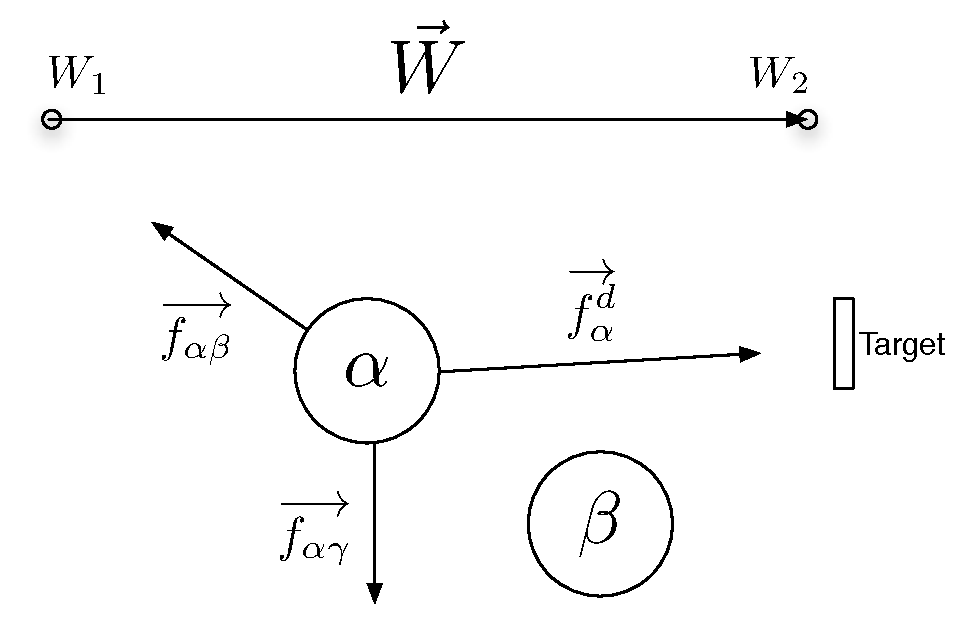
\includegraphics[scale=0.45]{Figures/ForceModel.pdf}} 
    \caption[Notation of forces acting on an agent]{Illustration of the forces acting on an agent $ \alpha $. $ \beta $ is another agent and the grey bar on the top represents a wall. $ \vec{f_{\alpha\beta}} $ is the repulsive force from agent $ \beta $, and $ \vec{f_{\alpha B}} $ is the repulsive force from the wall. $ \vec{f^{0}_{\alpha}} $ is a force that represents agent $ \alpha $'s desire to reach the exit.
    The x and y axes are defined by the Cartesian coordinate system.}
    \label{ForceModel}
\end{figure}

So far in the model it only mentioned the forces on the horizontal level, the gravitational force and normal force from the ground which works vertically are not mentioned at all.  The reason is that in this model they only consider the motion on the horizontal plane.  Since there is no motion vertically, the gravitational force and the normal force from the ground cancel each other.\\\\
\underline{The equation of motion for agent $ \alpha $:}\\

The general approach of the model to get the equation of motion follows the standard way. Summing up the forces acting on $ \alpha $ gives the acceleration, which builds the equation of motion. It comes in steps as the following.\\
First of all, the equation of motion deals with the agent $ \alpha $'s position $ \vec{r_{\alpha}} $, velocity $ \vec{V_{\alpha}} $, and acceleration $ \vec{f_{\alpha}} $. As the agent is not just a mass point, it has a radius $ r_{\alpha} $. The position and velocity vectors and the radius are shown in Figure \ref{NotationOfAgent}.

\begin{figure}[hb]
    \centering
    {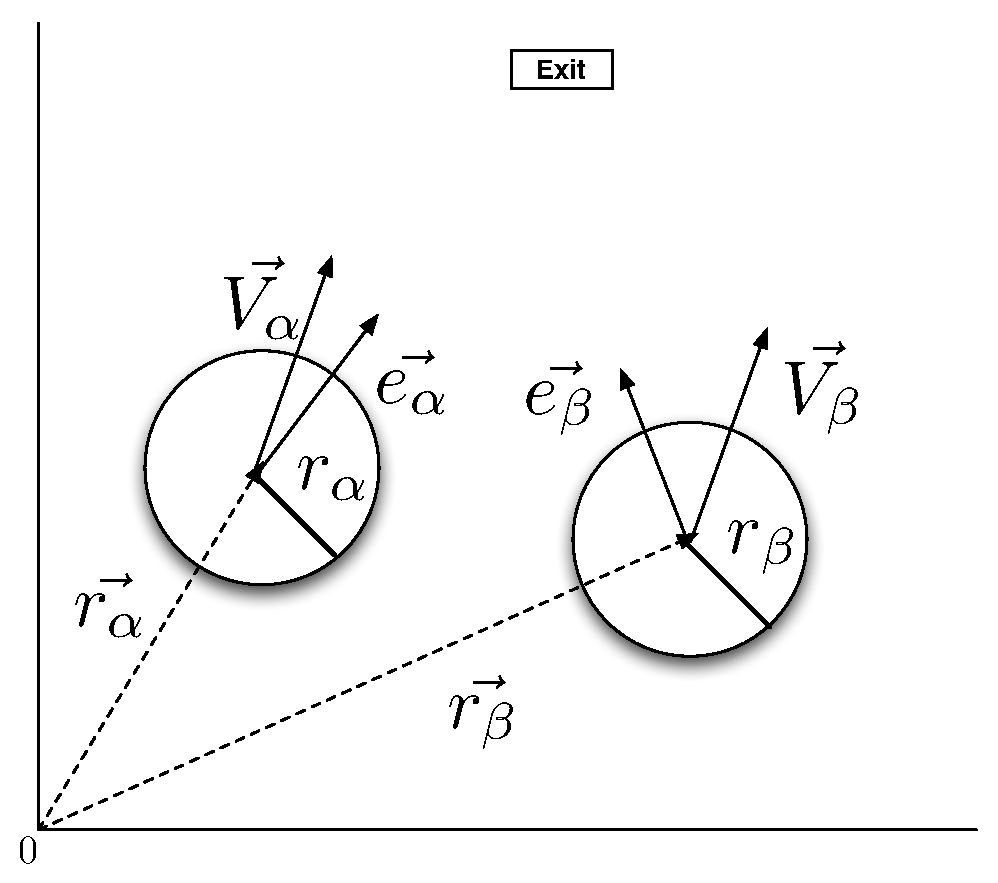
\includegraphics[scale=0.35]{Figures/NotationOfAgent.pdf}} 
    \caption[Notation of an agent]{Illustration of the visual presentation of the mathematical notations for position and velocity. As for agent $ \alpha $,
	    it has position vector $ \vec{r_{\alpha}} $, velocity vector $ \vec{V_{\alpha}} $, $\vec{e_{\alpha}}$ or $\vec{e_{\beta}}$ the normal vector pointing
	    to the exit and  $ r_{\alpha} $ or  $ r_{\beta} $ the radius of its body.
	    The x and y axes are defined by the Cartesian coordinate system.}
    \label{NotationOfAgent}
\end{figure}

The change in position $ \vec{r_{\alpha}} $ per time of 
agent $\alpha$ is actually the velocity $ \vec{V_{\alpha}} $:

\begin{equation}
		\frac{d \vec{r_{\alpha}}}{dt} = \vec{V_{\alpha}} \left( t \right)
\end{equation}

Also known from Newtonian physics, the change of velocity per time is the acceleration of agent $\alpha$, which is the result of a summation of all the forces acting on the agent, namely $\vec{f_{\alpha}} \left( t \right)$:

\begin{equation}
    \frac{d \vec{V_{\alpha}}}{dt} = \vec{f_{\alpha}} \left( t \right) 
\end{equation}

Referring to the part for force analysis, we need to add the driving force, repulsive force from the wall and repulsive force from other agents, also there is attractive force $ \vec{f_{\alpha i}} $ if the agent $ \alpha $ has some relatives or friends in the crowd.

\begin{equation}\label{model}
    \vec{f_{\alpha}} = \vec{f^{0}_{\alpha}} + \vec{f_{\alpha B}} +
    \sum_{\beta \neq \alpha} \vec{f_{\alpha \beta}} +  
    \sum_{i} \vec{f_{\alpha i}} 
\end{equation}

Naturally the work next is to show explicit expression for each force, and we will go through them one at a time explaining their mathematical structure and their role in the model.\\

\subsubsection{The driving force} %gotta figure out a better name for this part
The first term on the right hand side of equation \eqref{model} describes the implement of agent $ \alpha $'s "willingness" to reach the exit. In this model it is a velocity dependent force 
and is given by:

\begin{equation}\label{relaxtime}
	\vec{f^{0}_{\alpha}}\left( \vec{V_{\alpha}} \right) =
    \frac{1}{\tau}
    \left( V_{\alpha}^{0} \vec{e_{\alpha}} - \vec{V_{\alpha}} \right)
\end{equation}
where $V_{\alpha}^{0}$ is the desired speed, $ \vec{e_{\alpha}} $ is the normal vector pointing to the exit, $\vec{V_{\alpha}}$ is the actual velocity of the agent, and $\tau$ is the relaxation time. \\

From Equation \ref{relaxtime} we get the ideas that:
\begin{itemize}
\item About the notation, any quantity with a "$ ^{0} $ " on the upper right corner is a "desired" quantity.
\item Although $ \vec{f^{0}_{\alpha}} $ is a kind of desired force, it actually exists, because it appears in Equation \ref{model} for calculating the actual acceleration. However, the original article has not pointed out what is the source of  $ \vec{f^{0}_{\alpha}} $.  As the calculation of that force is closely related with the desired velocity $V_{\alpha}^{0}$, then we can think of the desired velocity as a imaginary source if we are not so interested in the physical source. We have considered the static frictional force as a most likely way of achieving the $ \vec{f^{0}_{\alpha}} $, and there are various other ways to fulfil that purpose, for example, by pulling.
\item $ V_{\alpha}^{0} \vec{e_{\alpha}} $ represent the desired velocity, which is needed to calculated in two steps, first to get the magnitude and then the direction. $ \vec{e_{\alpha}} $ is a normal vector pointing to the exit.
\item In Equation \ref{relaxtime}, $\tau$ is used to divide the difference between the desired velocity and the actual velocity. Equation \ref{relaxtime} fits dimensional analysis, because the quantity get from the division is some form of acceleration. 
\item Normally the relaxation time means the time needed to get from one state to another. The article \cite{self-org} suggests $ \tau_{\alpha}\approx 1s $, which shows that it usually takes the agent $ 1s $ to change its velocity.
\end{itemize}
The desired speed at some time $V_{\alpha}^{0}\left( t \right)$ is given by:

\begin{equation}\label{v0eta}
    V_{\alpha}^{0}\left( t \right) = \left[ 1 - \eta_{\alpha} \left( t \right) \right] 
    V_{\alpha}^{0} \left( 0 \right) +
    \eta_{\alpha} \left( t \right)V_{\alpha}^{\text{max}}
\end{equation}
where $V_{\alpha}^{0} \left( 0 \right)$ is the desired speed at $ t=0 $, and $V_{\alpha}^{\text{max}}$ is the maximum desired speed of agent
$\alpha$. \\
$\eta_{\alpha}$ is called the impatience or nervousness of the agent and is given by:

\begin{equation}\label{eta}
	\eta_{\alpha} \left( t \right) =
    1 - \frac{\overline{V}_{\alpha} \left( t \right)}
             {V_{\alpha}^{0} \left( 0 \right)}
\end{equation}
where $\overline{V}_{\alpha}\left( t \right)$ is the average speed in the desired direction.\\\\
As for Equation \ref{v0eta} and Equation \ref{eta}, we have the following considerations:
\begin{itemize}
\item The maximum desired speed $V_{\alpha}^{\text{max}}$ is the speed that agent $\alpha$ will try to get if it is allowed by the 
environment and other agents. 
\item The desired speed $V_{\alpha}^{0} \left( t \right)$ Changes with time, and especially varies with the impatience factor which is also a function of time $ t $.
\item The average speed $\overline{V}_{\alpha} \left( t \right)$ along the desired direction is not specified in the original article, and our understanding of that concept is as in Figure \ref{impatience}, where the projection( the projected vector is called $ \vec{r_{\alpha}^{E}}$ ) of $ \vec{r_{\alpha}} $ onto the desired direction of motion is used to calculate $\overline{V}_{\alpha} \left( t \right)$.

\begin{figure}[ht]
\centering
{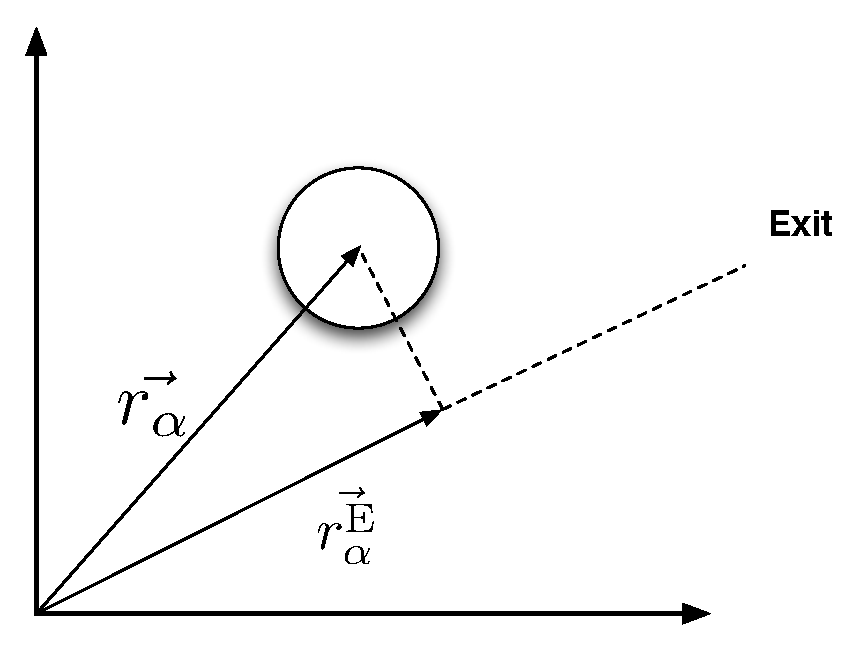
\includegraphics[scale=0.35]{Figures/NotationOfAgent2.pdf}} 
\caption{Illustration of the vector $ \vec{r_{\alpha}^{E}}$, which is the projection of $ \vec{r_{\alpha}} $ onto the desired direction of motion.}
\label{impatience}
\end{figure}

Therefore, we want to calculate $\overline{V}_{\alpha} \left( t \right)$ in the following way:
\begin{equation}\label{averagespeed}
   \overline{V}_{\alpha} \left( t \right) = \frac{1}{t} \vec{r_{\alpha}}\cdot \vec{e_{\alpha}} 
\end{equation}
\item From Equation \ref{v0eta} the initial desired speed $V_{\alpha}^{0} \left( 0 \right)$ is used to calculated desired speed at any time $ t $, and if we put $ t=0 $ into the equation, we have
\begin{equation}
    V_{\alpha}^{0}\left( 0 \right) = \left[ 1 - \eta_{\alpha} \left( 0 \right) \right] 
    V_{\alpha}^{0} \left( 0 \right) +
    \eta_{\alpha} \left( 0 \right)V_{\alpha}^{\text{max}}
\end{equation}
where $ \eta_{\alpha} \left( 0 \right) $ is not known.
Also for Equation \ref{eta}, put $ t=0 $ and we get
\begin{equation}
	\eta_{\alpha} \left( 0 \right) =
    1 - \frac{\overline{V}_{\alpha} \left( 0 \right)}
             {V_{\alpha}^{0} \left( 0 \right)}
\end{equation}
although the initial average speed $ \overline{V}_{\alpha} \left( 0 \right) $ is not defined in the original article, we decide to put $ \overline{V}_{\alpha} \left( 0 \right)=0 $, because in that case 
\begin{eqnarray}
	\eta_{\alpha} \left( 0 \right) &=&
    1 - \frac{\overline{V}_{\alpha} \left( 0 \right)}
             {V_{\alpha}^{0} \left( 0 \right)}\\
&=& 1 - \frac{0}{V_{\alpha}^{0} \left( 0 \right)}
= 1
\end{eqnarray}
which makes sense, as when the emergency suddenly happens our agent should feel extremely anxious ($ \eta_{\alpha} \left( 0 \right)=1 $). Then we know the initial desired speed $ V_{\alpha}^{0}\left( 0 \right) $ is
\begin{eqnarray}
    V_{\alpha}^{0}\left( 0 \right) &=& \left[ 1 - \eta_{\alpha} \left( 0 \right) \right] 
    V_{\alpha}^{0} \left( 0 \right) +
    \eta_{\alpha} \left( 0 \right)V_{\alpha}^{\text{max}}\\
&=& \left( 1 - 1 \right)  
    V_{\alpha}^{0} \left( 0 \right) +
    1 V_{\alpha}^{\text{max}}\\
&=& V_{\alpha}^{\text{max}}
\end{eqnarray}
\item Equation (\ref{v0eta}) and Equation (\ref{eta}) contains an intermediate variable $ \eta_{\alpha} \left( t \right) $, 
so in principle we are allowed to eliminate $ \eta_{\alpha} \left( t \right) $ and only show the 
relationship between $ V_{\alpha}^{0}(t) $ and $ \overline{V}_{\alpha} \left( t \right) $. Thus we get:

\begin{equation}\label{vv}
    V_{\alpha}^{0}(t) = \left[ 1 - \frac{V_{\alpha}^{max}}{V_{\alpha}^{0}(0)}\right]\overline{V}_{\alpha} \left( t \right) + V_{\alpha}^{max}
\end{equation}

\begin{figure}[ht]
\centering
{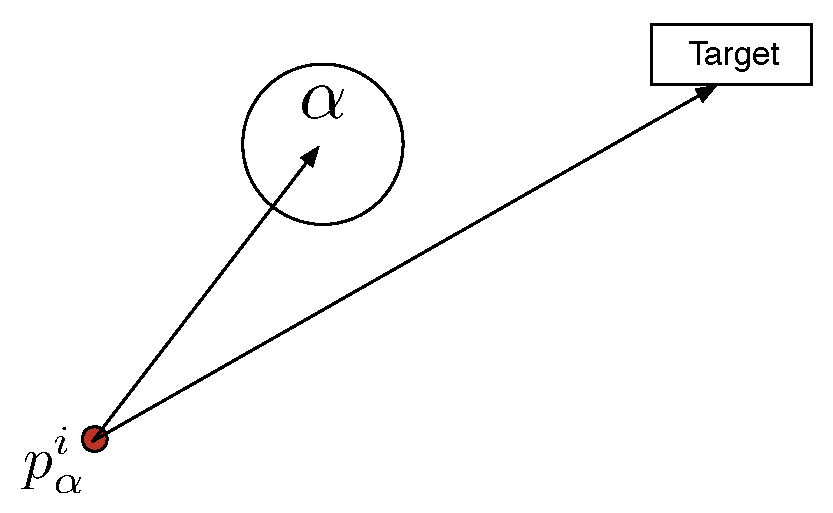
\includegraphics[scale=0.35]{Figures/impatience.pdf}} 
\caption[The impatience factor]{Illustration on the correlation between the function about the desired speed $ V_{\alpha}^{0}(t) $ 
and the average speed in the desired direction of motion $ \overline{V}_{\alpha} \left( t \right) $, and the graph of
$ V_{\alpha}^{0}(t) = \left[ 1 - \frac{V_{\alpha}^{max}}{V_{\alpha}^{0}(0)}\right]\overline{V}_{\alpha} \left( t \right) + V_{\alpha}^{max} $
intersects with the axis at $ \left( 0 , V_{\alpha}^{max} 
\right)  $ and $ \left(V_{\alpha}^{max} 
		\frac{V_{\alpha}^{0} \left( 0 \right) }{V_{\alpha}^{max}-V_{\alpha}^{0} \left(0 \right)} , 0 
\right)  $.
When $\alpha$'s velocity is at maximum the impatience gets low, and vice versa.}
\label{fig:impatience}
\end{figure}

Figure (\ref{fig:impatience}) is a drawing of the graph about those two variables, and the intersection
 of the function line with both axis are:

\begin{equation}
\left( 
	\overline{V_{\alpha}} , V_{\alpha}^{0} \left( t \right)
\right)
=
\left( 
	0 
		, 
	V_{\alpha}^{max} 
\right) 
\text{and} 
\left(
	V_{\alpha}^{max} 
		\frac{V_{\alpha}^{0} \left( 0 \right) }{V_{\alpha}^{max}-V_{\alpha}^{0} \left(0 \right)} 
	, 0 
\right) 
\end{equation}
Normally, the values of the two speeds should have positive values, so the graph is part of a straight line.
Now there is a doubt the range of the value of $ \overline{V}_{\alpha} \left( t \right) $, compared with $ V_{\alpha}^{max} $, 
if we have already 
set $ V_{\alpha}^{max} $ a fixed number for a certain agent. In the case:
\begin{equation}
	V_{\alpha}^{max} 
	\geq 
	V_{\alpha}^{max} 
	\frac{V_{\alpha}^{0}(0)}{V_{\alpha}^{max}-V_{\alpha}^{0}(0)}
\end{equation}
we get the relation:
\begin{equation}
V_{\alpha}^{0}(0)\leq \frac{1}{2} V_{\alpha}^{\text{max}}
\end{equation}
Which contradicts with our earlier conclusion that
\begin{equation}
    V_{\alpha}^{0}\left( 0 \right) = V_{\alpha}^{\text{max}}
\end{equation}
Therefore, the graph should not intersect with $ \overline{V_{\alpha}} $ axis under normal circumstances when the maximum desired velocity is not exceeded.
\item However, from Equation \ref{vv}  and Figure \ref{impatience} we think that $V_{\alpha}^{\text{max}}$ can be exceeded, but only under rare situations. For example, at $ t=0 $, if agent $ \alpha $ moves opposite to the exit because of some extreme large repulsive force, then from Equation \ref{vv} $ V_{\alpha}^{0} \left( 0 \right)  $ is larger than $V_{\alpha}^{\text{max}}$.
\item If there are no repulsive forces at all, the only source of acceleration is from the desired velocity, which modifies the actual velocity to the desired direction and value.  After some time, the actual velocity should reach some constant, which resembles the so called terminal velocity in physics when the acceleration is zero.  When the agent reaches the terminal velocity the actual velocity does not change and it equals the average velocity, so we can write the acceleration from Equation \ref{relaxtime} as

\begin{equation}
\vec{f}_{\alpha} = \vec{f^{0}_{\alpha}}\left( \vec{V_{\alpha}} \right)
\end{equation}
\begin{equation}
\frac{1}{\tau}\left( V_{\alpha}^{0} \vec{e_{\alpha}} - \overline{V}_{\alpha} \left( t\right) \vec{e_{\alpha}}  \right)  = 0
\end{equation}
As $ \tau $ is a constant, despite the direction of the velocity vector we have
\begin{equation}\label{terminal}
	 V_{\alpha}^{0} - \overline{V}_{\alpha} \left( t\right) 
    = 0
\end{equation}

Also we take Equation \ref{vv}, and insert the value of $ V_{\alpha}^{0}(t) $ from Equation \ref{vv} to Equation \ref{terminal}:

\begin{equation}
	\left[ \left( 1 - \frac{V_{\alpha}^{max}}{V_{\alpha}^{0}(0)}\right)\overline{V}_{\alpha} \left( t \right) + V_{\alpha}^{max} \right] - \overline{V}_{\alpha} \left( t\right) 
    = 0
\end{equation}
Solve for $ \overline{V}_{\alpha} \left( t\right) $ we get:
\begin{equation}
\overline{V}_{\alpha} \left( t\right) = V_{\alpha}^{0}(0)
\end{equation}
Which makes a lot of sense because the terminal velocity is the initial desired velocity and equals the maximum desired velocity.

\item The impatience or nervousness factor is active when one calculates the 
force action on agent $\alpha$ from the velocity of the agent.

In the case where $0 \leq \eta_{\alpha} \leq 1$ the expression for 
$V_{\alpha}^{0} \left( t \right)$  makes sense. Here we can see why this term 
is called the impatience of the agent. If the fraction  between the average 
speed in the desired direction and the initial speed is low then $\eta_{\alpha} \approx 1$. 
When the impatience term is close to one $V_{\alpha}^{0} \left( t \right)$ 
is dominated by $V_{\alpha}^{\text{max}}$. That is, if the agent have not 
moved very far in the desired direction compared to the initial speed the 
impatience of the agent will cause the agent's future velocity to be dominated by 
the desired velocity of the agent.

If the agent has been moving in the desired direction with his initial 
speed the entire time then $\eta_{\alpha} = 0$  and 
$V_{\alpha}^{0} \left( t \right)$ will continue to be $V_{\alpha}^{0} \left( 0 \right)$.

In the case where $\eta_{\alpha} \leq 0$ that is the agent has moved further 
in the desired direction then he would have had he been walking with his 
initial speed. The expression for $V_{\alpha}^{0} \left( t \right)$
stats yield strange results. That $\eta_{\alpha} \leq 0$ would imply that:

\begin{equation}\label{n}
    V_{\alpha}^{0} \left( t\right) = \left[ 1 + \eta_{\alpha} \left( t \right) \right] 
    V_{\alpha}^{0} \left( 0 \right) -
    \eta_{\alpha} \left( t \right)V_{\alpha}^{\text{max}}
\end{equation}

And this will yield a negative value for $V_{\alpha}^{0}$ if: 

\begin{equation}
\left[ 1 + \eta_{\alpha} \left( t \right) \right] 
V_{\alpha}^{0} \left( 0 \right) < \eta_{\alpha} \left( t \right)V_{\alpha}^{\text{max}} 
\end{equation}

This is a problem because it is not that far fetched that an agent will be 
forced to exceed his desired velocity.

In the case where $1 \leq \eta_{\alpha}$ it would mean that the agent has moved 
further in the opposite direction than the desired one and this can only happen very 
weird situations.
\end{itemize}

% Lets have a little summation here. What have we learned about the inpatience factor and
% the velocity dependant force. What kind of dynamics does this force yield





\subsubsection{Repulsion from the walls}
Now the second term on the right hand side of \eqref{model} is a force which arise from interactions with the walls or other obstacles. The forces, caused by the wall or obstacles, is given by:

\begin{equation}\label{wallpotential}
    \vec{f_{\alpha B}} \left( \vec{r_{\alpha}} \right) =
    - \nabla_{\vec{r_{\alpha}}} U_{B}
    \left( \| \vec{r_{\alpha}} - \vec{r_{B}^{\alpha}} \| \right)
\end{equation}
$U_B$ is a repulsive potential and $ \| \vec{r_{\alpha}} - \vec{r_{B}^{\alpha}} \|$ is the distance 
from the position of agent $\alpha$ to the nearest point $ \vec{r_{B}^{\alpha}}  $ of the wall and shown in figure \ref{NotationOfWall}.

\begin{figure}[ht]
\centering
{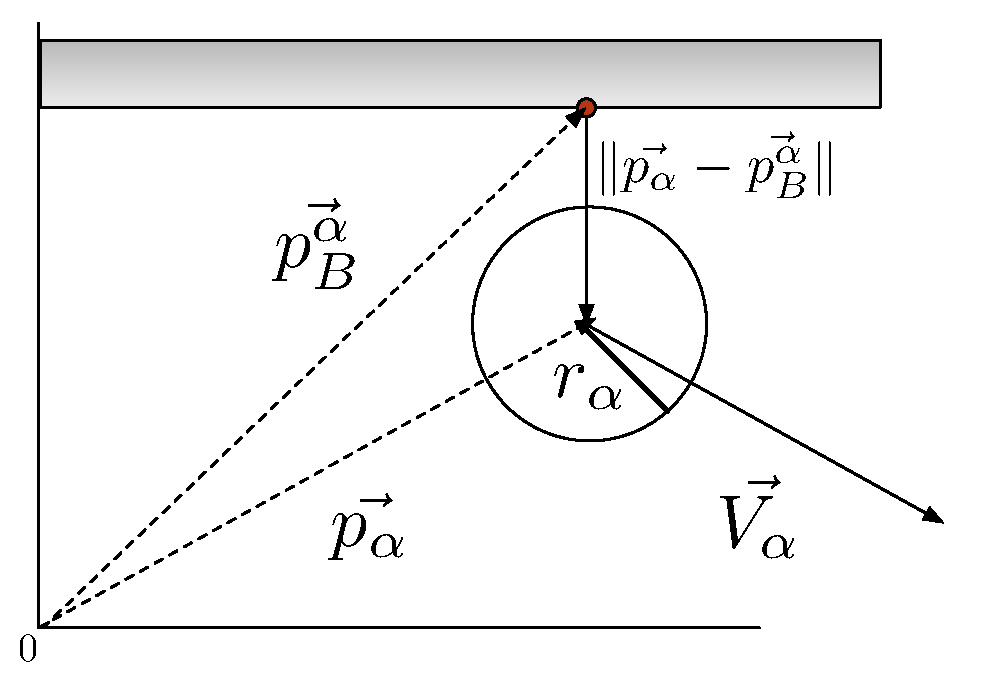
\includegraphics[scale=0.35]{Figures/NotationOfWall.pdf}} 
\caption[Notation of the interaction between an agent and a wall]{The illustration shows the mathematical notation for the interaction with walls used. The circle is pedestrian $\alpha$ with radius $r_{\alpha}$, $\vec{r_{\alpha}}$ is the position vector for $\alpha$, the grey box on the top is the wall, $\vec{r_{B}^{\alpha}}$ is the position vector for the closest part of the wall to $\alpha$, $\left( \| \vec{r_{\alpha}} - \vec{r_{B}^{\alpha}} \| \right)$ is the smallest distance from $\alpha$ to the wall and $\vec{V_{\alpha}}$ is the velocity vector for $\alpha$.}
\label{NotationOfWall}
\end{figure}

\begin{itemize}
\item  $U_B$ only depends on the distance $ \| \vec{r_{\alpha}} - \vec{r_{B}^{\alpha}} \|$, so the gradient of $V_B$ tells us in which direction does this distance change the most. It is obvious that the changes is largest if the agent takes a step directly towards or away from the wall, which means that the agent will always be pushed directly away from the wall.

\item The next job is to find an explicit expression for $ \| \vec{r_{\alpha}} - \vec{r_{B}^{\alpha}} \|$\\
To start of with we need to find point on the wall that is perpendicular to $\alpha$ as it will be the nearest.  
If we define the wall as a vector, $\vec{W}$ going from a point in space $w_1$ to another point $w_2$, then we can find the projection of $\alpha$ onto the wall and this projection will be $\vec{r_{B}^{\alpha}}$.
The equation for the projection is
\begin{equation}\label{wall}
\vec{r_{B}^{\alpha}}=\frac{\vec{r_{\alpha}}\cdot \vec{W}}{\| \vec{W} \|^2}\vec{W}
\end{equation}
With this we now have the two points we need to calculate $ \| \vec{r_{\alpha}} - \vec{r_{B}^{\alpha}} \|$.


\item With the explicit expression for $ \| \vec{r_{\alpha}} - \vec{r_{B}^{\alpha}} \| $, we are able to calculate $ \vec{f_{\alpha B}} \left( \vec{r_{\alpha}} \right) $ from Equation \ref{wallpotential}, if the expression for the potential function $ V_{B}
    \left( \| \vec{r_{\alpha}} - \vec{r_{B}^{\alpha}} \| \right) $ is given.\\
In some of the other articles [ ] made by the same outhers as the article which makes the basis for the model in this repport, the repulsive potential from the wall is given as
\begin{equation}
U_{B} \left( \| \vec{r_{\alpha}} - \vec{r_{B}^{\alpha}} \| \right) =
U^0_{\alpha B} e^{- \| \vec{r_{\alpha}} - \vec{r_{B}^{\alpha}} \| / r_{\alpha} }
\end{equation}
where $U^0_{\alpha B}$ is a constant and $r_{\alpha}$ is the radius of a pedestrian $\alpha$. \\

In that case, the wall repulsive force on agent $ \alpha $ is:
% TODO: make \begin{equation} and \begin{slpit}. This is a general thing for all \begin{allign}
\begin{equation}
    \vec{f_{\alpha B}} \left( \vec{r_{\alpha}} \right) =
    - \nabla_{\vec{r_{\alpha}}} U_{B}
    \left( \| \vec{r_{\alpha}} - \vec{r_{B}^{\alpha}} \| \right)\\
=-\left( \frac{\partial}{\partial x_{\alpha}}U_{B}( \| \vec{r_{\alpha}} - \vec{r_{B}^{\alpha}} \|), \frac{\partial}{\partial y_{\alpha}}U_{B}( \| \vec{r_{\alpha}} - \vec{r_{B}^{\alpha}} \|)\right) \\
\end{equation}
Calculating the derivatives we get 
\begin{equation}
    \vec{f_{\alpha B}} \left( \vec{r_{\alpha}} \right) 
=-\left(\left(U^0_{\alpha B}\frac{1}{r_{\alpha}}\frac{e^{- \| \vec{r_{\alpha}} - \vec{r_{B}^{\alpha}} \| / r_{\alpha} } (x_{\alpha}-x_B^{\alpha})}{\| \vec{r_{\alpha}} - \vec{r_{B}^{\alpha}} \| }\right),\left(U^0_{\alpha B}\frac{1}{r_{\alpha}}\frac{e^{- \| \vec{r_{\alpha}} - \vec{r_{B}^{\alpha}} \| / r_{\alpha} } (y_{\alpha}-y_B^{\alpha})}{\| \vec{r_{\alpha}} - \vec{r_{B}^{\alpha}} \| }\right)\right) \\
\end{equation}

\item The exponential function will always lay between 0 and 1:
\begin{equation}
0 < e^{ -\| \vec{r_{\alpha}} - \vec{r_{B}^{\alpha}} \| /r_\alpha} < 1
\end{equation}
Which leads to
\begin{equation}
0< U_{B} \left( \| \vec{r_{\alpha}} - \vec{r_{B}^{\alpha}} \| \right) < U^0_{\alpha B}
\end{equation}
We can see that this force act in the following way:\\
$\vec{f_{\alpha B}}$ tends to 0 as the distance $ \| \vec{r_{\alpha}} - \vec{r_{B}^{\alpha}} \|$ gets large, meaning that a pedestrian in a reasonably distance from the wall will feel a diminishing force. $\vec{f_{\alpha B}}$ tends to $V^0_{\alpha B}$ as the distance $ \| \vec{r_{\alpha}} - \vec{r_{B}^{\alpha}} \|$ tends to $0$ the pedestrian will be pushed, with some force depending on $V^0_{\alpha B}$, away from the wall. 
The negative of the force means that when the potential between wall and pedestrian rises so will the force, but in the opposite direction meaning that the pedestrian will be pushed away. This can be understood as if the pedestrian is trying to avoid the wall as it is expected from real life situations.
 [Helbing and Molnár, 1995]. %real references, please.
\end{itemize}

 
\subsubsection{Repulsion from other agents}
The third term on the right hand side of \eqref{model} is a summation of all the 
force between agent $\alpha$ and agent $\beta$. It is a function of the position vector and the velocity of 
both agents, and it is given by:

\begin{equation}
    \sum_{\beta \left( \neq \alpha \right)}
        \vec{f_{\alpha \beta }}\left( t \right) =
        A_{\alpha}^{1} exp \left(
            \frac{ r_{\alpha \beta} - d_{\alpha \beta }}
                 {B_{\alpha}^1}
        \right)
    \vec{\eta_{\alpha \beta}} \cdot
    \left(
        \lambda_{\alpha} + \left(
            1 - \lambda_{\alpha}
        \right)
		\frac{1+\cos{\phi}}{2}
    \right) +
    A_{\alpha}^{2} exp\left(
        \frac{r_{\alpha \beta} - d_{\alpha \beta}}
             {B_{\alpha}^{2}}
    \right)
    \vec{\eta_{\alpha \beta}}
    \label{agentinteraction}
\end{equation}

\begin{figure}[ht]
    \centering
    {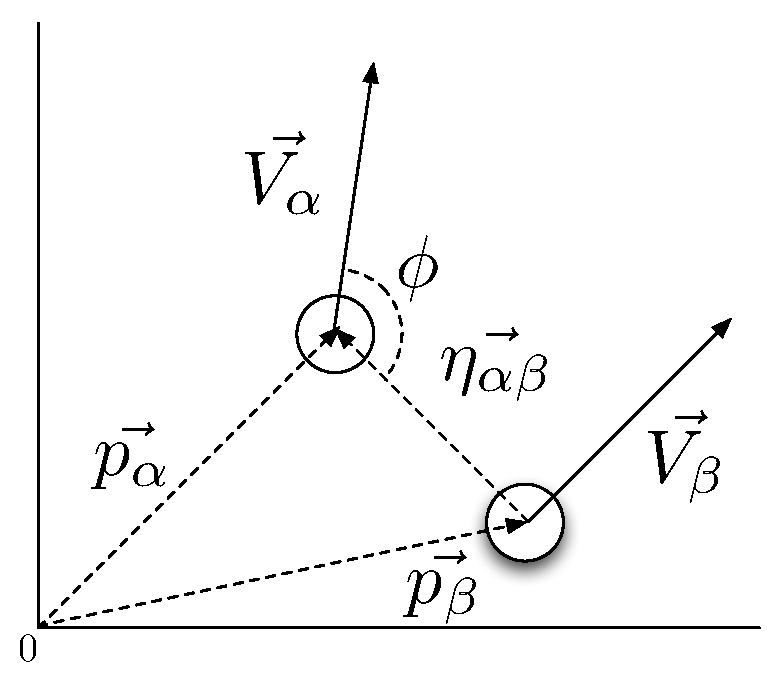
\includegraphics[scale=0.35]{Figures/NotationOfInteraction.pdf}} 
    \caption[Notation of the interaction between two agents]{Illustration of the notation for the interaction between agents.
	     An addition and difference to \ref{NotationOfWall} is that the wall has been replaced by pedestrian $\beta$.
	     $\eta_{\alpha \beta}$ is the normal vector pointing from $\alpha$ to $\beta$, and $\phi$ is the angle between $\alpha$'s 
	     velocity vector and $\beta$'s center of mass.}
    \label{NotationOfInteraction}
\end{figure}

Here $A_{\alpha}^{1}$, $A_{\alpha}^{2}$, $B_{\alpha}^{1}$, $B_{\alpha}^{2}$ 
and $\lambda_{\alpha}$ are all constants that can differ for each agent. 
$r_{\alpha \beta}$ is the sum of the radii of $\alpha$ and $\beta$ that is 
$r_{\alpha \beta} = r_{\alpha} + r_{\beta}$. $d_{\alpha \beta}$ is the 
distance from the center of mass of agent $\alpha$ and the center of mass of 
agent $\beta$ and is therefore given by $d_{\alpha \beta} = 
\|\vec{r_{\alpha}}\left( t \right) - \vec{r_{\beta}}\left( t \right) \|$.
$\eta_{\alpha \beta}$ is the normal vector pointing from $\alpha$ to $\beta$ 
and it is given by:

\begin{equation}
    \eta_{\alpha \beta} =
        \frac{\vec{r_{\alpha}}(t) - \vec{r_{\beta}}(t)}
             {\|\vec{r_{\alpha}}(t) - \vec{r_{\beta}}(t) \|}
\end{equation}

the angle $\phi$ in \eqref{agentinteraction} is the angle between the normal 
vector pointing from agent $\beta$ to $\alpha$ and the direction in which 
agent $\alpha$ is moving. Cosine to the angle is 

\begin{equation}
\cos \left( \phi \right)
	\left( t \right) 
		= 
	- \vec{\eta_{\alpha \beta}}
		\left( t \right) 
	\cdot 
\vec{e_{\alpha}}\left( t \right)
\end{equation}

Equation \eqref{agentinteraction} is divided into two terms. The first term on 
the right hand side reflects the agents tendency to stay at a certain distance 
from other agents. This part of the force is called the private sphere because 
the agent prefers to have some free space around him if possible. The radius 
of the private sphere can differ from agent to agent. The constant 
$A_{\alpha}^{1}$, $B_{\alpha}^{1}$ and $\lambda_{\alpha}$ control the nature 
of the private sphere $A_{\alpha}^1$ and $B_{\alpha}^1$ control the strength 
and range of the interaction respectively. $\lambda_{\alpha}$ is there to take 
into account a persons tendency to focus on things happening in front of him 
rather than behind him.	% we should make a drawing of this.

The second term of equation \eqref{agentinteraction} deals with physical interaction.
In the situation where the density of the crowd is high the agents will have be closer
to each other and the social sphere is undermined. % go more into detail here 
So if we look away from the social sphere for a minute and concentrate on the physical
interaction we will see that if we omit the social sphere the calculation will be reduced to
to:

\begin{equation}\label{re}
\overrightarrow{f_{\alpha\beta}}(t) = A_{\alpha}^{2} exp\left[ \frac{r_{\alpha\beta} - d_{\alpha}\beta}{B_{\alpha}^{2}}\right]  \overrightarrow{n_{\alpha\beta}}
\end{equation}

Taking the norms of both sides of Equation (\ref{re}), we can draw the relation between the value of $\overrightarrow{f_{\alpha\beta}}(t)$ and $ d_{\alpha\beta} $, as shown in Figure 
(\ref{physicalinteraction}).\\

\begin{figure}
    \centering
    {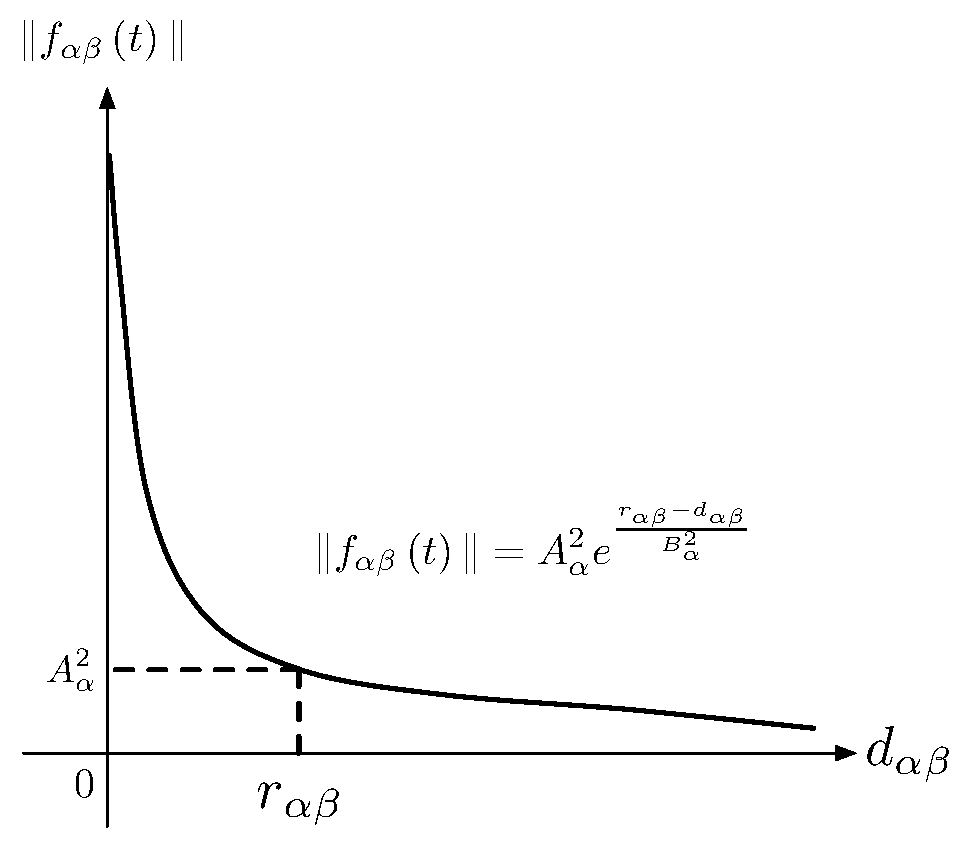
\includegraphics[scale=0.45]{Figures/physicalinteraction.pdf}} 
    \caption[Psysical interaction]{Illustration of the function about the interaction force 
        $f_{\alpha\beta}(t)$ and the distance between two agents
        $d_{\alpha \beta}$. It follows that the smaller the distance between two agents, the greater the interaction force is. }
    \label{physicalinteraction}
\end{figure}

There is one intersection of the graph and the  axis at:

\begin{equation}
	\left( d_{\alpha \beta} , \| \vec{f_{\alpha \beta}} \left( t \right) \| \right)
 =
	\left( 0 , A_{\alpha}^{2} exp\left( \frac{r_{\alpha\beta} }{B_{\alpha}^{2}}\right)  \right) 
\end{equation}

If put into the constants, we will be able to get a maximum value of $ f_{\alpha\beta}(t) $, 
since the distance between agents cannot be negative. Here we set $ A_{\alpha}^{2} = 3 m/s^{2} $, 
$ r_{\alpha\beta} = 0.6 m $, and $ B_{\alpha}^{2} = 0.2 m $, so 
$ f_{\alpha\beta}(t)^{max} \doteq 60 m/s^{2} $, which is about six times the gravitational 
acceleration and represents a rather large force between agents (as large as six person's weight).

However, we notice that the effective part of the force calculated above is only the horizontal 
component that enables the agent to move horizontally in the plane where we do the simulation, 
but the reality is that the agents sometimes are also able to move vertically, for example, 
by stepping upon other people when they cannot take the pushing force from the surrounding agents. 
When that happens, the horizontal component of the repulsive force becomes smaller even if $ d_{\alpha\beta} $ 
is kept the same.	

\begin{figure}[ht]   
\centering
    {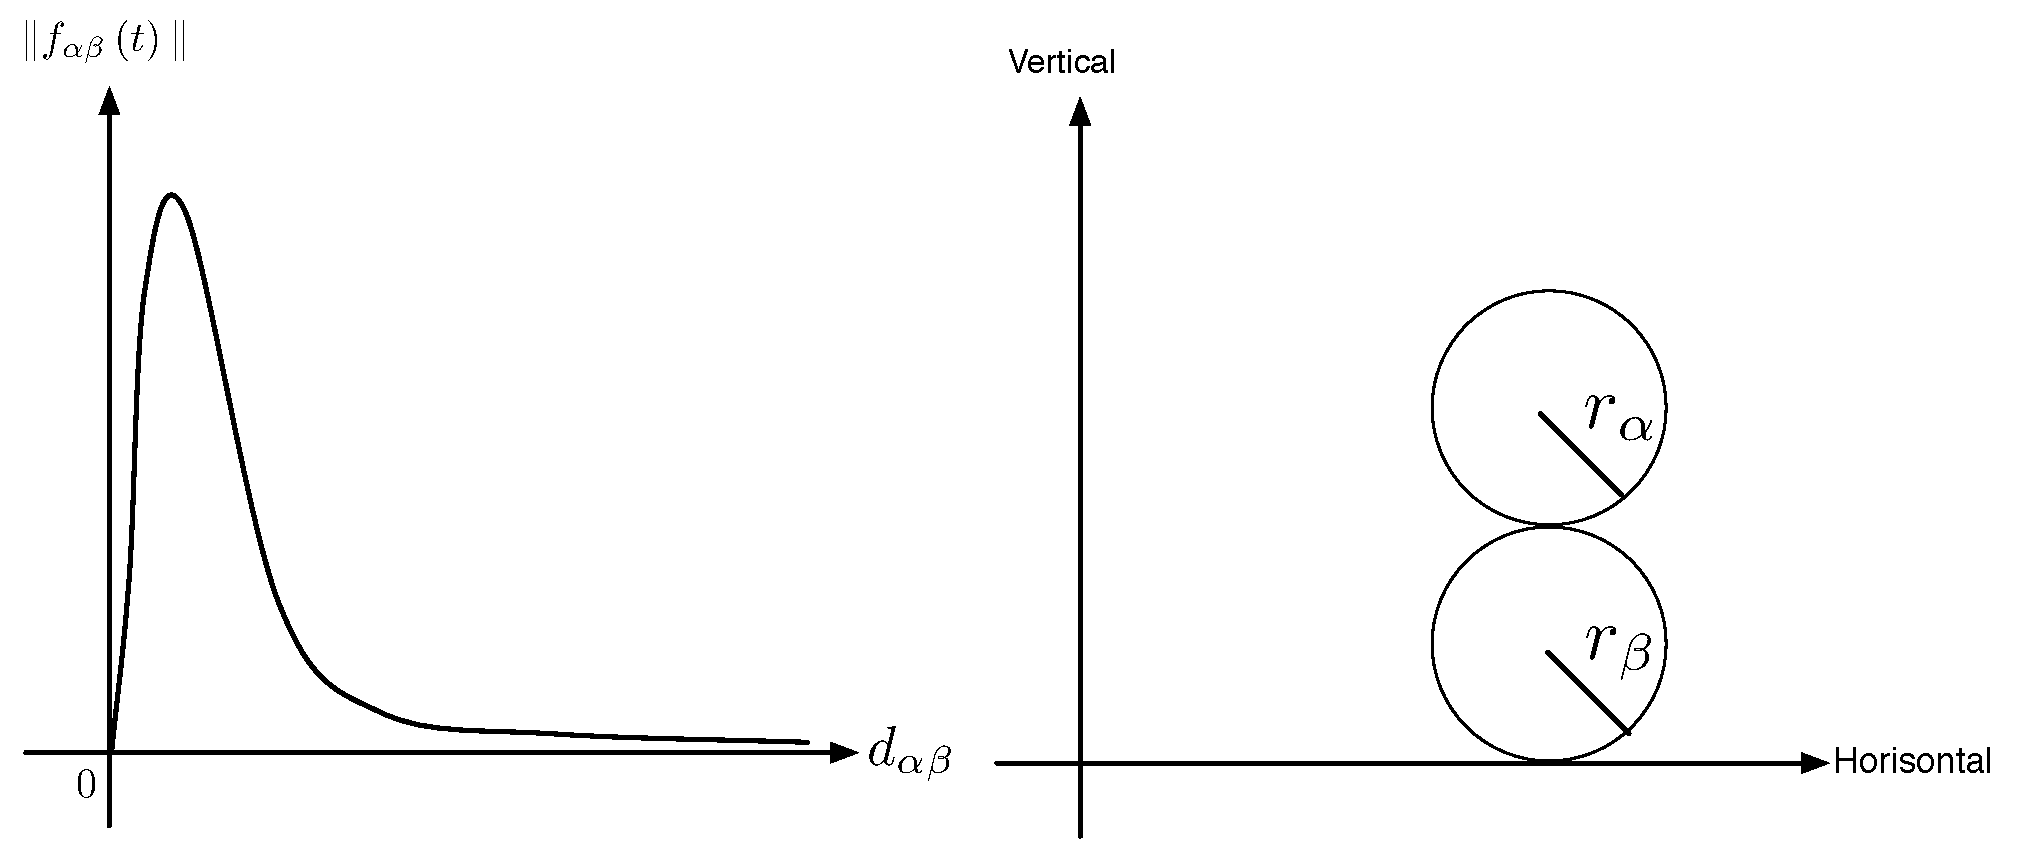
\includegraphics[scale=0.35]{Figures/ForceOverlapping.pdf}} 
    \caption{}
    \label{forceoverlapping}
\end{figure}

Therefore, a qualitative modification of dependence between $ f_{\alpha\beta}(t) $ and $ d_{\alpha\beta} $ could be:
% remember to finish this section

% again lets  have a little summation here. What kinds of dynamics does the
% social interaction part of the model yield.

\subsubsection{The attractive forces between some agents}
The fourth and last term in \eqref{model} represents the force from attraction 
in the room. Attractions can be either be either interesting sculptures or 
sights or familiar persons the agent prefer to be close to, such as friends 
and family. The mathematical structure of this force is the same as the force 
from other agents, however it is opposite in algebraic sign and has different 
constants. 

To get an overview of how the model is put together look a figure \ref{overview}
with the aid of table \ref{tableofconstandvar}

\begin{figure}[hb] %with some more comments i think that this figure could serve as a summation of the entire section
    \centering
    {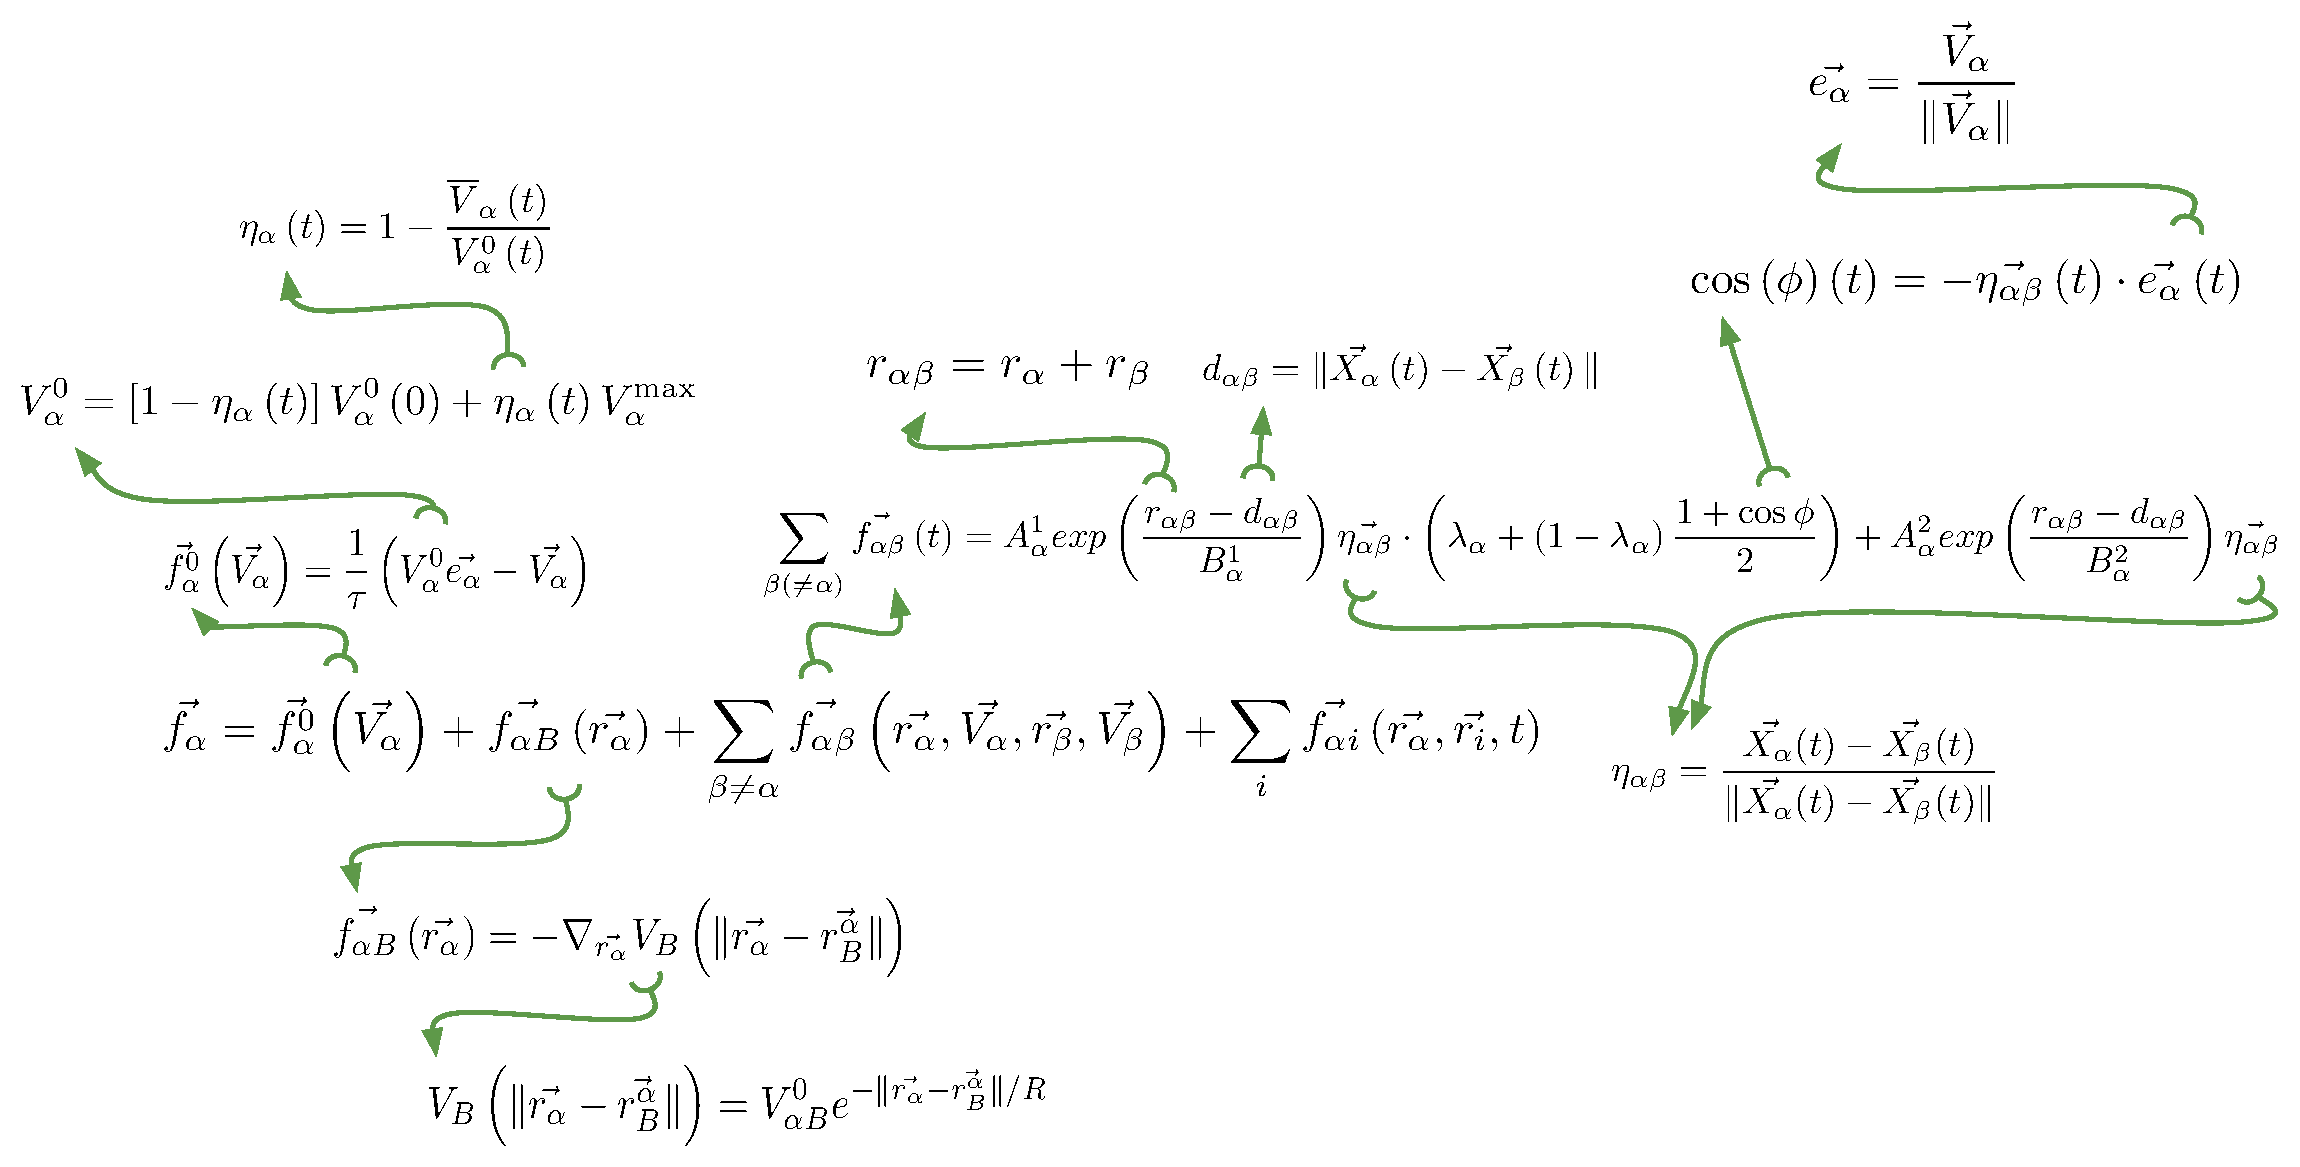
\includegraphics[scale=0.45]{Figures/overview.pdf}} 
    \caption[Overview of the model]{Illustration of an overview of how the model is put together. The different equations and their notation is written to give the 
	     reader an overview of how the model looks like.}
    \label{overview}
\end{figure}
\clearpage
\section{Lack of features in the model}

\label{sec:lack}
When we started to implement the model and simulate our two cases, we encountered some
problems that we did not foresee when we read the article \cite{self-org}, and the other
articles \cite{helbing00}, \cite{social-force}.
We encountered some special cases where the model did not suffice to give a realistic
simulation, and also we could not, from the articles, figure out how to fix some initial parameters.
In the articles the authors did not write of any such problems and how to deal with them,
so we had to come up with our own solutions to solve them, and thereby give a more realistic
simulation.
In the following section we discuss these problems and our solutions to these problems.

\subsection{Discussion on walls in special cases.}\label{wallEndpoints}
The wall is created as a vector. The repulsive force vector is perpendicular to the wall 
vector and has a direction directly towards the pedestrian $\alpha$.

In the general case of the repulsive force on an agent, $\alpha$, from a wall 
nearby is given as a function of the vector from the nearest point. This point we 
calculate by finding the point that makes the vector form $\alpha$ to the wall be 
perpendicular to to vector that is the wall. In some cases though the point will not 
be on the wall it self. This of course makes no sense since the agent would then be 
repulsed by a non existing part of the wall meaning that it would avoid free 
areas. In this case we would have to use the end point of the wall. But doing this 
can make some unrealistic behaviour as well, if the walls have the right composition. 

Let's start out by looking at a case with no problem. A case with no problems is a 
room where the angles between the walls is less than $180^o$, i.e. a squared room 
where the angles are $90^o$. For a pedestrian close to the corner between two walls, we 
would calculate the repulsive force from both of the walls. By doing this, we can avoid 
the agents to go through either one of the walls. Then we get a force directly away 
from each of the walls. This clearly makes sense and there is no problem in doing so.

\subsubsection{Forces at kinks}
The case where the angle between two walls is greater than $180^o$ could on the 
other hand give some problems if not handled correctly. The case is sketched in 
figure \ref{fig:wallcase}. Here there are 3 different areas that a pedestrian $\alpha$ 
can be in. The area A where $\alpha$ is only perpendicular to wall $1$, in area B, 
$\alpha$ will not be perpendicular to any of the walls and in C he will be only 
perpendicular to wall 2. 

If a pedestrian is in area B then we would calculate the 
forces from the end point of the walls. This will be from the point where the two 
walls meet. This will give a double repulsion from one point and that 
does not make sense. Also when the agent is in are A or C it would get a repulsive force 
from a second wall it would be of no risk of going into and in many situations 
could not see because the first wall is blocking the sight. This of course does not 
make any sense either. So the way that we handle this situation is the following. 
When the angle between the walls is greater than $180^o$, from agent $\alpha$'s 
point of view, it should look at the two walls as one, and in that way it will 
only calculate one force from the walls. In area A or C only the closest point 
on the closest wall should affect it. In the case of $\alpha$ being in area B 
the walls themselves does not matter, only the vector going from the conjoint 
point of the walls to $\alpha$, should affect and only one time. Doing this, 
there should be no unrealistic scenarios concerning wall junctions and walls 
with more than $180^o$ between them. But this could create undesired 
behaviour at doors of other objects created with free end points.

\begin{figure}[ht]
\centering
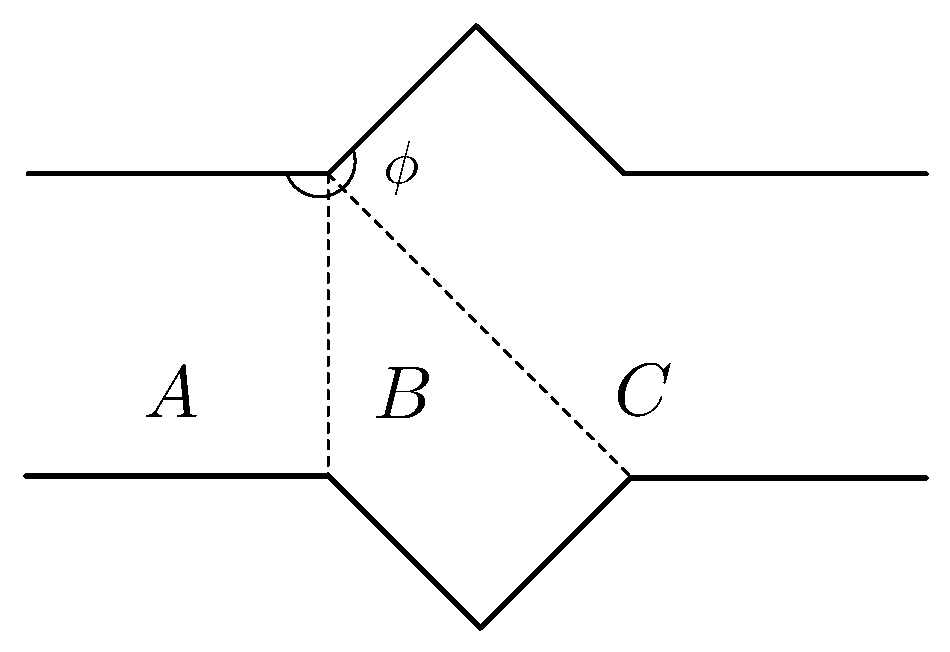
\includegraphics[scale=0.45]{Figures/WallCase.pdf} 
\caption{}\label{fig:wallcase}
\end{figure}

\subsubsection{The force at doorways}
We encountered a problem when dealing with doors. The problem arises because 
the door is constructed by two free endpoints and an agent feels two repulsion 
forces from these points according to section \ref{wallEndpoints}. This means 
that a pedestrian trying to exit through the door will feel repulsive forces 
from both of the walls which prevent it from walking through the door. The moment it 
passes through the door it will be pushed forward and accelerate which is unwanted 
behaviour. This we resolved by removing the force from free endpoint when:

\begin{equation}
\| p - w \| > R
\end{equation}
where $ p $ is the position of the agent, $ w $ is the position of the door's endpoint, 
and $ R $ is the radius of the agent.

This creates what we could call a "non repulsion zone" see figure(Mikkel Lav Tegning!).
In rare cases it could happen that an agent is trying to exit the room and it feels 
no repulsion because it is in the "non repulsive zone", and it is then pushed sideways out 
of the "non repulsion zone" and suddenly it will feel a great repulsive force because 
it first "discovers" the force when it is very close to the wall see figure(Mikkel Lav Tegning!).

\subsubsection{Calculating the repulsion from walls}
\label{sec:repulsion-points}
The calculation of repulsion from the walls is split in two parts for each 
agent: First all the points on the walls that will affect the agent is 
identified, then the repulsion from each point is calculated. As explained in 
section~\ref{sec:the-model}, the repulsion from the wall is measured from the 
nearest point of the wall to the actor. Identifying these points is done using 
the following algorithm:

\begin{enumerate}
    \item For each wall, calculate the projection of the vector pointing from 
        the wall's starting point to the agent, unto the vector pointing from 
        the wall's starting point to its endpoint.
        \begin{enumerate}
            \item If this point is part of the wall, save it to the list of points 
                repulsion should be calculated from, and add the wall's two endpoints 
                to the list of already used endpoints.

            \item If the projected point is not part of the wall, the endpoint closest 
                to the agent is used instead. This endpoint is saved to a 
                third list of endpoints repulsion should be calculated from.
        \end{enumerate}

    \item After having gone through all walls, for each point in the third 
        list, check if this point is already in the list of used endpoints. If 
        so, discard it. Otherwise, add it to the list of points repulsion 
        should be calculated from, and to the list of used endpoints.
\end{enumerate}

The algorithm starts out with the list of walls, and produces a list of points 
to calculate this repulsion from, ensuring that no wall endpoint is used 
twice. The points are then used as a basis for calculating the repulsion, as 
described in section~\ref{sec:the-model}.

\subsection{Initial conditions and constants}
\label{sec:init-cond}
% TODO: Go through all the constants and add where we got it from; either a 
% reference or saying that we came up with it ourselves.
When initialising the model, parameters are set for each agent. In the 
model, every parameter can vary between actors, while in practice many of them 
do not. In this section, we go through the parameters and how they are set.  
For all random numbers, the operating system's built-in random number 
generator is used and considered to be sufficient for our purposes. We run 
multiple simulations of the same initial conditions by fixing the seed of the 
random number generator to the same value for each run. Distributions are 
drawn by using the distribution functions of the \emph{NumPy} mathematical 
library for Python \cite{numpy}.

\subsubsection{Position related parameters}
There are a number of parameters that are set that have to do with the initial 
position of actors and walls. Some are given, and some we had to come up
with ourselves. They are:

\begin{itemize}
    \item \textbf{Wall endpoints:} Points describing the endpoints of the 
        walls. They are set according to the scenario we want to simulate, so 
        in a square room with a single exit in the middle of a wall, there 
        will be five wall segments.

    \item \textbf{Agent positions:} Each agent has a starting position 
        distributed randomly within the room. They are created by drawing a 
        set of random numbers for the x and y coordinates respectively, and 
        adjusting the range of this random number to be within the room's 
        dimensions. Agents' positions are adjusted so that they do not overlap 
        with the walls by adjusting coordinates so that the distance from the 
        center of each agent to each wall is at most the radius. This 
        adjustment is not made between agents, so they may overlap initially. 
        It is assumed that the model will correct this within the first few 
        simulation steps, which is also what we have seen in practice.

    \item \textbf{Agent's radius:} The agent's radius is drawn from a normal 
        distribution with a mean of $0,3$ meters and a standard deviation of 
        $0,05$ meters. This is done to simulate a natural variety in the width 
        of human shoulders, and to avoid deadlocks caused by perfectly 
        symmetrical forces that might otherwise occur \cite{helbing00}.
        %TODO: Check this reference, maybe better explanation?
\end{itemize}

\subsubsection{Movement related parameters}
A number of parameters are set to control the movement of the agents. They 
are:

\begin{itemize}
% TODO: Add a section about placement of waypoints.
%   Square room: Place the waypoint at or just outside the exit.
%   Corridor: Place the waypoint a long distance away, so that pedestrians 
%   move almost in a straight line along the corridor.
    \item \textbf{Waypoint:} We think of this setup that suits each scenario  
        by ourselves. Each agent has a waypoint that they move towards, 
        and is the same for all agents when there is only one exit. 
        For a square room, this waypoint is set just outside the exit the agent 
        will move towards. For a corridor, the waypoint is put at a position 
        far away from the corridor and along the line that the corridor lies, so that
        there is no traffic rules for each agent such as to stick to the right or left.
        
        %where there are multiple exits, actors are set to move towards one of 
        %the exits at random, regardless of their position within the room. 
        Since the model does not deal with pathfinding, waypoints are not 
        changed during the simulation. When an agent reaches its waypoint, it is 
        considered to have escaped, and is removed from the simulation.

    \item \textbf{Initial velocity:} The initial velocity does not matter much 
        because the agent can quickly adjust its velocity during the first few 
        step sizes, and there is no recommends from the articles. 
        Our way of getting the initial velocity is by setting both a vector and a scalar 
        representing vector length. The scalar velocities are drawn from a 
        normal distribution with a mean of $1.34$ and a standard deviation of 
        $0,26$. The initial velocity vectors are created by multiplying the 
        scalar velocity with a normalised vector pointing from the agent's 
        initial position to the waypoint.
        % TODO: Where do the mean and deviation come from?

    \item \textbf{Desired speed $  V_{i}^{0}  $:} The desired speed is 
        the speed the agent wants to move at (see the explanation in 
        section~\ref{sec:the-model}). The desired speed at $ t=0 $ is set 
        equal to the initial speed 
        under our assumption that when people start to leave a room they will 
        initially (try to) move with their desired speed, and then be 
        affected by the model parameters once they start moving.

    \item \textbf{Maximum desired speed $ V_{i}^{max} $:} The maximum 
        desired speed depends on its desired speed as $ V_{i}^{max} =1.3 V_{i}^{0}  $.
       c
        
    \item \textbf{Relaxation time $ \tau $:} The relaxation time is the time it would 
        take an unhindered agent to adjust to its desired velocity after 
        having been hindered by something blocking their path. This is set to 
        one second for all actors, in \cite{self-org}. However, in another article 
        \cite{helbing00}, the relaxation time is $ 0,5 $.

    \item \textbf{$\lambda$:} \cite{ABconstant} chose $\lambda$ $\approx 0.1$ 
        to take into account
    anisotropic character of pedestrian interaction, such that the situations 
    in front of
    a pedestrian have bigger impact on the pedestrians behaviour than things 
    going on
    behind them. 
    % TODO: Is this explanation correct?
\end{itemize}

\subsubsection{Constants} \label{constants}
The model includes a number of constants. These are parameters that do not 
vary between the agents, but are fixed for the whole simulation. They are:

\begin{itemize}
    \item \textbf{Timestep:} The timestep is the $\Delta t$ that passes for 
        each step of the simulation. As discussed in 
        section~ %TODO: Make new reference
		, there are various trade-offs in making 
        this parameter larger or smaller. We have experimented with different 
        values, and have found that a value of $0,01$ seconds makes for a 
        simulation without errors such as jitter that results from larger 
        timestep values. Since setting the timestep corresponds to setting a 
        delta value for an Euler integration, there are various methods that 
        originate from this integration method, that might be used to vary the 
        timestep dynamically during the simulation. 
         However, we have found 
        that with a fixed value of $0,01$ seconds, we get reasonable 
        performance of our simulation, so we have not found the need to 
        complicate our program by applying such methods.
        % TODO: Reference for dynamic timestep adjustment

    \item \textbf{$A$, $B$:} These values are given in \cite{ABconstant}. 
        Although the model allows for them to vary between agents, we have 
        (just as is done in the article) set them to a fixed value for the 
        whole simulation. The values given are $A_2=3,0$ and $B_2 = 0,2$.

    \item \textbf{$ U^{0} $:} While calculating the wall repulsive force, a potential
        constant $ U^{0} $ is needed to get the force. Though it will be realistic to 
        have a hard core potential \cite{self-org}, we have tried different values 
        of $ U^{0} $ so that the agents do not keep a too far distance from the wall 
        and they do not pass through the wall under normal conditions. In the end, 
        we choose $ U^{0} =2 $ .
 
\end{itemize}


\clearpage
% vim:ft=tex
\section{Simulation approach}
\label{sec:simulation}
In this section, we describe how our simulation is implemented, and how the 
implementation works. This is done in part to document our implementation, and 
in part to give the reader an overview of how our results are obtained.
We will describe briefly how the program is structured on a macro level, and 
go into more detail on the parts specific to the calculations of the model 
parameters. The full source code is available online\footnote{See 
\url{http://akira.ruc.dk/~tohojo/crowd-modelling}.}.

Our simulation is implemented in the Python programming language, with the 
calculation intensive parts implemented in C for performance reasons. We 
assume a virtual coordinate system using meters as a base unit, and with the 
origin in the centre of the area we simulate. Each pedestrian is 
described by a centre point and a radius, and each wall is described by a line 
segment connecting two points.

All parameters are stored as double precision floating point values where 
nothing else is indicated. We use custom data structures to keep track of the 
pedestrians and walls while running the simulation. Python is used to set up the 
initial conditions, run the program's main control loop, and draw the 
simulation results through the \emph{PyGame} library \cite{pygame}. This 
allows to do real-time animation as well as saving each simulation step 
to be assembled into a film afterwards. All calculations and data processing 
is done in a Python extension written in C, to increase performance. Gathering 
of data to draw the graphs and the drawing itself is done in the Python code. 

\subsection{Structure of the program}
The program is structured into four main parts: The simulation calculations, 
drawing of the simulations, plotting of parameters and the control part 
setting up parameters and calling the other parts as necessary. The drawing 
part mainly consists of a frontend to the drawing library, and so is not 
interesting to discuss here. The other parts will be described in the 
following, structured so as to present the sequence that is followed when a 
simulation is run. This description consists of three parts: setting up the 
simulation, calculations, and gathering of results.

\subsection{Setting up the simulation}
The program supports defining multiple \emph{scenarios} to simulate. Each 
scenario defines its own set of parameters, and a simulation run features one 
scenario. The parameters defined for each scenario include:

\begin{itemize*}
    \item The model constants, $A$, $B$, $U$, $\lambda$ and pedestrian relaxation 
        time. These are the same for all pedestrians in a simulation.
    \item Mean initial desired velocity and radius of pedestrians and their standard 
        deviation, and the factor used to calculate the maximum velocity.
    \item The initial number of pedestrians, the area(s) they start in and the 
        target(s) they move towards.
    \item The geometry of the scenario (i.e. placement of walls).
    \item Definition of the areas where measurement of data for plotting 
        graphs is done and which parameters should be plotted (see 
        section~\ref{sec:measurement}).
    \item Various parameters related to drawing of the simulation, maximum run 
        time and optional continuous inflow of pedestrians.
\end{itemize*}

Parameters that are not set for each scenario, but are defined once for all 
simulations are:

\begin{itemize*}
    \item Time step size.
    \item Plotting data sampling frequency.
\end{itemize*}

How the values of the parameters are determined is described in 
section~\ref{sec:init-cond}. From these parameters, the simulation is set up 
by initialising the calculation module and creating the pedestrians.

The pedestrians are created with an initial velocity of zero, and distributed 
randomly within the area(s) designated by the parameters for the scenario, as 
described in section~\ref{sec:init-pedestrians}. 

\subsection{Calculation of the model}
\label{sec:model-calculation}
For each step of the simulation, the calculations are run in two parts: 
Finding the accelerations (or resulting force) for all pedestrians, and 
updating position and velocity for the pedestrians.  Since the acceleration 
for each pedestrian is dependent on both position and velocity of the other 
pedestrians, splitting the calculations this way enables us to do the 
calculations of pedestrians in any order, and even parallel. The drawback 
is that the pedestrians are only affected by the movement and positions of 
other pedestrians as they were at the end of the last simulation step. This 
means that the time step has to be small enough that this doesn't matter in 
practice.

The acceleration vectors for each pedestrian, $\alpha$, is calculated in three 
steps, corresponding to the parts $\overrightarrow{f_\alpha^d}$, 
$\overrightarrow{f_{\alpha \beta}}$ and $\overrightarrow{f_{\alpha \gamma}}$ from 
section~\ref{sec:the-model}. In each simulation step the three forces are 
calculated in order, first calculating the desired force, then the repulsive 
force from each of the other pedestrians in the simulation, and finally the 
repulsive force from each wall. The resulting vectors are added to yield the 
total acceleration for each pedestrian.

After this is calculated for all pedestrians, their velocities and positions are 
updated in separate steps. Each of these four steps are described in detail 
in the following. The code calling the other parts of the calculation can be 
seen in code segment~\ref{lst:calling}. This function is called once for each 
pedestrian (index \texttt{i}) for each simulation step.

\begin{lstlisting}[caption={Main function calling the other parts of the 
    calculation code.},label=lst:calling]
void calculate_forces(Py_ssize_t i)
{
    int j;
    add_desired_acceleration(&pedestrians[i]);

    for(j = 0; j < a_count; j++) {
        if(i == j) continue;
        add_repulsion(&pedestrians[i], &pedestrians[j]);
    }

    add_wall_repulsion(&pedestrians[i]);
}
\end{lstlisting}

\subsubsection{Calculating the desired force}
The function for calculating the desired force can be seen in code 
segment~\ref{lst:desired-force}. Of note is the implementation on lines 7-19 
of the conditional definition of $V_\alpha^d(t)$ given in 
equation~\eqref{eqn:cond-define} and the creation of a unit vector in lines 
20-21 to add the direction to the desired velocity.

To increase performance, it is preferred to update values in place, instead of 
copying them around in different parts of the computer's memory. This gives 
rise to the constructs around the \texttt{vector\_i*}-functions in the code; 
here the \emph{i} stands for ``in place''.

\begin{lstlisting}[caption={Calculating the desired 
    force.},label=lst:desired-force]
static void add_desired_acceleration(Pedestrian * a)
{
    double average_velocity = 0.0, impatience = 0.0, 
           desired_velocity = 0.0;
    Vector desired_direction = {0.0, 0.0};

    if(a->time) {
        double proj = vector_projection_length(
                a->initial_position, a->target, a->position);
        average_velocity = proj / a->time;

        impatience = 1.0 - average_velocity / a->initial_desired_velocity;

        desired_velocity = (1.0-impatience) * a->initial_desired_velocity + \
                           impatience * a->max_velocity;

    } else {
        desired_velocity = a->initial_desired_velocity;
    }
    desired_direction = vector_sub(a->target, a->position);
    vector_unitise(&desired_direction);

    a->acceleration = vector_mul(desired_direction, desired_velocity);
    vector_isub(&a->acceleration, &a->velocity);
    vector_imul(&a->acceleration, 1.0/a->relax_time);
}
\end{lstlisting}

\subsubsection{Repulsion from other pedestrians}
The two functions used for calculating the repulsion from other pedestrians is seen 
in code segment~\ref{lst:pedestrian-repulsion}. The \texttt{add\_repulsion} function 
is called for each pair of pedestrians. The force without any angle dependence is 
calculated in the \texttt{calculate\_repulsion} function, and is modified by 
the angular dependence if the pedestrian's velocity is not zero, and $\lambda$ is 
not one. If the velocity is zero, calculating the dot product would result in 
a division by zero, and if $\lambda$ is one, modifying the force by the 
angular dependence would have no effect. The whole calculation is skipped if 
one of the constants $A$ or $B$ are zero, as this would make the calculations 
have no effect, or result in a division by zero, respectively.

\begin{lstlisting}[caption={Calculating the repulsion from other 
    pedestrians.},label=lst:pedestrian-repulsion]
Vector calculate_repulsion(Pedestrian * a, Pedestrian * b, double A, double B)
{
    double radius_sum = a->radius + b->radius;
    Vector from_b     = vector_sub(a->position, b->position);
    double distance   = vector_length(from_b);

    vector_unitise(&from_b);
    vector_imul(&from_b, A * exp((radius_sum-distance)/B));

    return from_b;
}

void add_repulsion(Pedestrian * a, Pedestrian * b)
{
    if(!A || !B) return;
    Vector repulsion = calculate_repulsion(a, b, A, B);
	if(a->velocity.x && a->velocity.y && lambda < 1.0) {
		Vector from_a = vector_sub(b->position, a->position);

		double cosine = vector_dot(a->velocity, from_a)/(
				vector_length(a->velocity) * vector_length(from_a));

		vector_imul(&repulsion, (lambda + (1-lambda)*((1+cosine)/2)));
	}
    vector_iadd(&a->acceleration, &repulsion);
}
\end{lstlisting}

\subsubsection{Repulsion from walls}
The code for adding the repulsion from the walls is shown in code 
segment~\ref{lst:wall-repulsion}. The \texttt{add\_wall\_repulsion} function 
is called for each pedestrian and consists of two parts: Finding the points on the 
walls where repulsion should be calculated from, and calculating the repulsion 
from these points. The force from the repulsion points is calculated in the 
function \texttt{calculate\_wall\_repulsion} that is called for each repulsion 
point. This calculation corresponds to equation~\eqref{eqn:wall-repulsion}.

\begin{lstlisting}[caption={Calculating the repulsion from the 
    walls.},label=lst:wall-repulsion]
void add_wall_repulsion(Pedestrian * a)
{
    int i;
    Vector * repulsion_points  = PyMem_Malloc(w_count * sizeof(Vector));
    int rep_p_c = 0;
    Vector repulsion;

    rep_p_c = find_repulsion_points(a, repulsion_points);

    for(i = 0; i < rep_p_c; i++) {
        repulsion = calculate_wall_repulsion(a, repulsion_points[i]);
        vector_iadd(&a->acceleration, &repulsion);
    }


    PyMem_Free(repulsion_points);
}

Vector calculate_wall_repulsion(Pedestrian * a, Vector repulsion_point)
{
    Vector repulsion_vector = vector_sub(a->position, repulsion_point);
    double repulsion_length = vector_length(repulsion_vector);
    vector_unitise_c(&repulsion_vector, repulsion_length);

    double repulsion_force = (1/a->radius) * U * exp(-repulsion_length/a->radius);

    vector_imul(&repulsion_vector, repulsion_force);

    return repulsion_vector;
}
\end{lstlisting}

The function for finding the repulsion points on the walls is seen in code 
segment~\ref{lst:repulsion-points}. This is an implementation of the algorithm 
described in section~\ref{sec:repulsion-points}. Lines 9-27 corresponds to 
step one in the algorithm description that identifies definite repulsion 
points (those that are not wall endpoints) and possible repulsion points 
(those that are endpoints).

In lines 29-35 an endpoint is discarded if it is already used because it is 
shared with a wall that has already defined a repulsion point. In lines 36-57 
endpoints that are not discarded in this way are added to the list of 
repulsion points if they are either not free-floating (i.e. shared with 
another wall), or closer to the pedestrian centre than the pedestrian's 
radius. This ensures that doorways do not repulse pedestrians that are passing 
through it.

\begin{lstlisting}[caption={Finding the wall repulsion 
    points.},label=lst:repulsion-points]
int find_repulsion_points(Pedestrian * a, Vector repulsion_points[])
{
    int i,j;
    double projection_length;
    Vector * used_endpoints     = PyMem_Malloc(2*w_count * sizeof(Vector));
    Vector * possible_endpoints = PyMem_Malloc(w_count * sizeof(Vector));
    int rep_p_c = 0, use_e_c = 0, pos_e_c = 0;

    for(i = 0; i < w_count; i++) {
        Wall w = walls[i];
        projection_length = vector_projection_length(w.start, w.end, a->position);
        if(projection_length < 0)  {
            possible_endpoints[pos_e_c++] = w.start;
        } else if(projection_length > w.length) {
            possible_endpoints[pos_e_c++] = w.end;
        } else {
            // We have the length, L, of how far along AB the projection point is.
            // To turn this into a point, we multiply AB with L/|AB| and add
            // this vector to the starting point A.
			// P = A + AB*L/|AB|
            repulsion_points[rep_p_c++] = vector_add(w.start, 
                    vector_mul(vector_sub(w.end, w.start), 
                        projection_length/w.length));
            used_endpoints[use_e_c++] = w.start;
            used_endpoints[use_e_c++] = w.end;
        }
    }

    for(i = 0; i < pos_e_c; i++) {
        int use_e = 1;
        for(j = 0; j < use_e_c; j++) {
            if(vector_equals(possible_endpoints[i], used_endpoints[j])) {
                use_e = 0;
            }
        }
        if(use_e) {
			// Keep track of whether the endpoint is free-floating, i.e. if
			// it is shared with another wall.
			int free_e = 1;
			for(j = 0; j < pos_e_c; j++) {
				if(i != j && 
						vector_equals(possible_endpoints[i],
							possible_endpoints[j])) {
					free_e = 0;
				}
			}
			// Endpoints that are free-floating (i.e. sides of doorways) are
			// only considered for repulsion if they are closer to the pedestrian
			// than the pedestrian's radius. This allows pedestrians to pass more
			// freely through doorways.
			if(!free_e || 
					vector_length(vector_sub(a->position,
							possible_endpoints[i])) < a->radius) {
				repulsion_points[rep_p_c++] = possible_endpoints[i];
				used_endpoints[use_e_c++] = possible_endpoints[i];
			}
        }
    }

    PyMem_Free(used_endpoints);
    PyMem_Free(possible_endpoints);

    return rep_p_c;
}
\end{lstlisting}

\subsubsection{Updating position and velocity}
After every pedestrian has been updated with a resulting acceleration vector from 
the current simulation step, all pedestrians update their position and velocity.  
The position is updated by calculating a displacement vector as explained in 
section~\ref{sec:continuous-movement}.

After updating the position, the pedestrian's velocity is updated by adding 
the acceleration vector, to be used for the next simulation step. The code 
that does this is seen in code segment~\ref{lst:update-position}. Line 14 is 
related to the measuring of data for plotting, and will be explained in 
section~\ref{sec:measurement}.

\begin{lstlisting}[caption={Updating the pedestrian 
    position.},label=lst:update-position]
void update_position(Pedestrian * a)
{
	Vector delta_p = vector_add(
			vector_mul(a->velocity, timestep), 
			vector_mul(a->acceleration, 0.5 * pow(timestep, 2)));

    vector_iadd(&a->position, &delta_p);
	a->velocity = vector_add(a->velocity,
			vector_mul(a->acceleration, timestep));
    a->time += timestep;

    check_flowlines(a);
}
\end{lstlisting}

\subsection{Obtaining results}
\label{sec:measurement}
There are two ways we obtain results from the simulation: through the drawings 
of the simulations themselves, and through graphs of various measurements made 
during the simulation. In this section we describe the mechanisms for 
obtaining these results. Which results are used for which scenarios are 
described, along with the scenarios themselves, in section~\ref{sec:results}.

\subsubsection{Drawings of the simulation}
When the simulation is run, drawings of the pedestrian's positions, walls etc. are 
created for each simulation step. These can be shown in real time, or saved 
and either assembled into a film or used as individual illustrations. We use 
these images to make qualitative assessments of pedestrian behaviour, e.g. 
determining whether a lane formation occurs. We include the relevant images as 
illustrations in the results section.

\subsubsection{Graphs of measurements}
As part of the simulation program, we have added measurements of various 
properties of the simulation, which are then assembled into graphs after the 
simulation has run. This section describes the measuring features we have 
added to the program, and \emph{how} they work. \emph{Why} we measure each 
property is explained along with the results. Since we have revised which 
graphs are needed throughout our work with the simulations, some additional 
measuring and graphing features exist in the source code, but are not 
described here.

The graphing functionality works in two different modes: One is graphing 
properties as a function of the simulation time, and others run multiple 
simulations varying one or more parameters and graphing properties as a 
function of this varied parameter. Any numeric parameter can be varied in this 
way. It is noted for each feature in which mode it is used and some properties 
are used for both modes. The properties we measure are:

% TODO: Pros and cons of these measurements.

\begin{itemize}

    \item \textbf{Flow rate:} Flow rate is measured along a line segment 
        defined as a parameter to the scenario; the line segment is assumed to 
        be perpendicular to the primary movement direction of the pedestrians.  
        The simulation keeps track of at what time each pedestrian first comes 
        into contact with this line segment, i.e. is first less than their 
        radius away from it . This is used as an approximation of when the 
        pedestrians cross the line. The average flow rate is then computed as 
        the number of pedestrians who have crossed the line divided by the 
        time.  This is graphed as a function of time, using a five second 
        moving average, and as a function of parameters, using the average of 
        the flow rate measurements of an entire simulation.

    \item \textbf{Leaving time:} The leaving time is a measure of how long it 
        takes for all pedestrians to leave the simulation completely. Pedestrians are 
        removed from the simulation when they reach their target, or when they 
        get outside the calculation area which is the basis of this 
        measurement. This property is only measured for a whole simulation, 
        and as such is only graphed as a function of the varying parameters. 
        Of course simulations that do not have a finite running time (i.e. 
        where pedestrians are added continuously, or where they never reach their 
        target) do not measure this property.
\end{itemize}

\subsection{Summary}
In this section we have described our implementation of the simulation. The 
program is split up into three parts: setting up the simulation with 
parameters and initial conditions, the calculations of the model itself, and 
measurements of the results. The first and last parts are implemented in the 
Python programming language, while the calculations themselves are implemented 
in C for performance reasons. The measurements of simulation results include 
drawing of pictures of the simulation, and graphs of the flow rate and the 
time it takes all pedestrians to leave a room.

\clearpage
\section{Results}
\label{sec:results}
In this section we describe the results obtained from our simulations. We have simulated two scenarios: A square room where the pedestrians exit through a single door, and pedestrians walking through a corridor where there is a bidirectional flow. For each scenario we describe the parameters we have set for the scenario, which features we found worth measuring for this scenario, the results we expected, and the results we obtained. Possible remedies for any discrepancies between the expected and the actual results are discussed in section~\ref{sec:discussion}.

\subsection{Constants}
We will here shortly specify the values for the different constants we use in both of the scenarios.
In the simulation the parameters are set after \cite{ABconstant} and \cite{self-org}, to see if we can replecate their simulations and results.
The general values we use are


\begin{itemize*}
    \item Strenght of pedestrian repulsion $A= 3,0$. 
    \item Range of pestrian repulsion $B: 0,2$.  
    \item Anisotropic constant $\lambda: 0,1$.
    \item Wall constant $U: 2.0$.
    \item Mean desired velocity: $1,34 m/s$, deviation $0,26 m/s$. Max velocity factor $1,3$.
    \item Mean radius of pedestrians $0,3 m$, deviation $0,05 m$.
    \item Relaxation time: $1,0 s$.
    \item Number of pedestrians: $100$.
\label{Table_constants}
\end{itemize*}

We will through the chapter mension when the values are changed for a specific case. 

\subsection{The square room scenario}
In this scenario we simulate pedestrians leaving a square room of 10 m by 10 m with a single $80cm$ wide door. 100 pedestrians are positioned randomly throughout the room. The second the simulation start all pedestrians head for the exit. The parameters for this simulation are as in \ref{Table_constants}

First the claim of the "faster-is-slower" effect is tested.
\begin{quote}
Even counterintuitive
effects are well reproduced. This includes the “faster is-
slower effect” and stripe formation in intersecting flows. \cite{self-org}
\end{quote}
We would then expect that a high nervousness would lead to slower evacuation, because of additional clogging at the doorway. But this phenomena do not occur in our simulation see figure \ref{FastIsSlow}
\begin{figure}
\centering
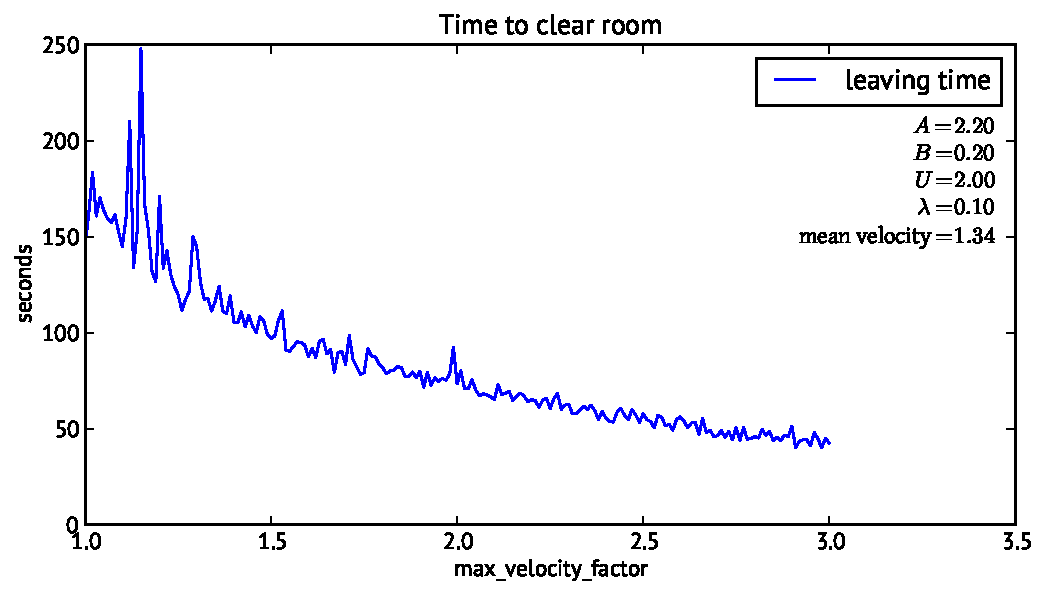
\includegraphics[scale=0.5]{Figures/fastIsSlowNot}
\caption{Fast is not slow}
\label{FastIsSlow}
\end{figure}
The larger the nervousness the faster is the evacuation. We have increased the max-velocity factor sow much that people eventually move through the walls. This start occurring around max-velocity-factor = 2.5, and measurements beyond this point are neglected.

Pedestrian flow rate is measure in the door opening, and the density of pedestrians in a 2 m by 2 m area directly in front of the door is measured. We also measure the time it takes for all pedestrians to leave the room.

The parameters for this simulation are the ones shown in \ref{Table_constants}

% TODO: Add parameters that are varied.


\subsection{The corridor scenario}
In this scenario we simulate pedestrians walking in both directions along a 20 
m long and six metres wide corridor. The pedestrians are divided into two 
groups, starting in opposite ends of the corridor and moving towards each 
other. The targets the pedestrians move towards are set 500 metres to each 
side, to make pedestrians walk in almost a straight line instead of converging 
towards the middle of the corridor. Flow rate is measured in the middle of the 
corridor, as is density. We start out with 100 pedestrians, adding a 
continuous inflow of three pedestrians per second, to simulate people arriving 
from outside the simulated area. Both the initial placement and the inflow of 
pedestrians are distributed randomly (i.e. approximately evenly) between the 
two ends of the corridor.

We expect to see lane formations through out our simulations
and the freezing by heating effect when we start raising the mean velocity
of the agents.

\subsubsection{Intial conditions and relaxation time $1,0$ second}

The parameters for this simulation are as in \ref{Table_constants} with the exception of the pedestrians
\begin{itemize*}
    \item Number of pedestrians: $50$ starting, adding $3/s$.
\end{itemize*}

When running the simulation we observe lane formations, and they almost clog up
in the corridor.

When we do a simulation with the max velocity factor set to $4.0$, instead of the normal $1.3$, the clogging
that occurs in the beginning eases up, and the pedestrians relatively fast
get out of the clogging and continuous toward their target. In this simulation
we also observe lane formations.

\begin{figure}[h]
\centering
\subfloat[The figure show the density in corridor when the parameters are set as \cite{ABconstant} and \cite{self-org}.]{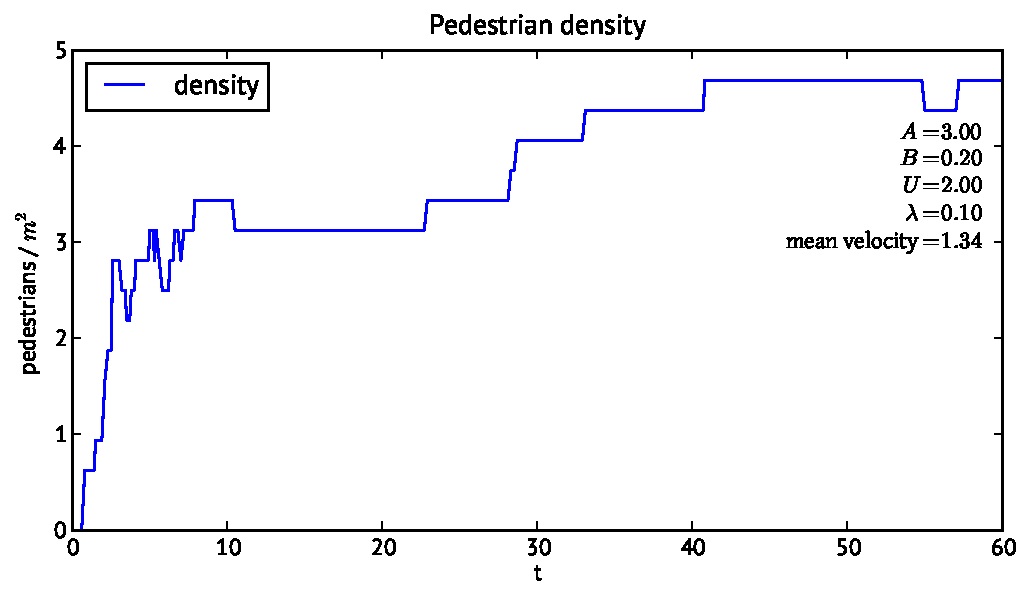
\includegraphics[scale=0.45]{Figures/dens_init_relax1.pdf}}
\subfloat[This figure shows the density in the corridor when the max velocity factor is set to $4.0$, and the other parameters as figure a.]{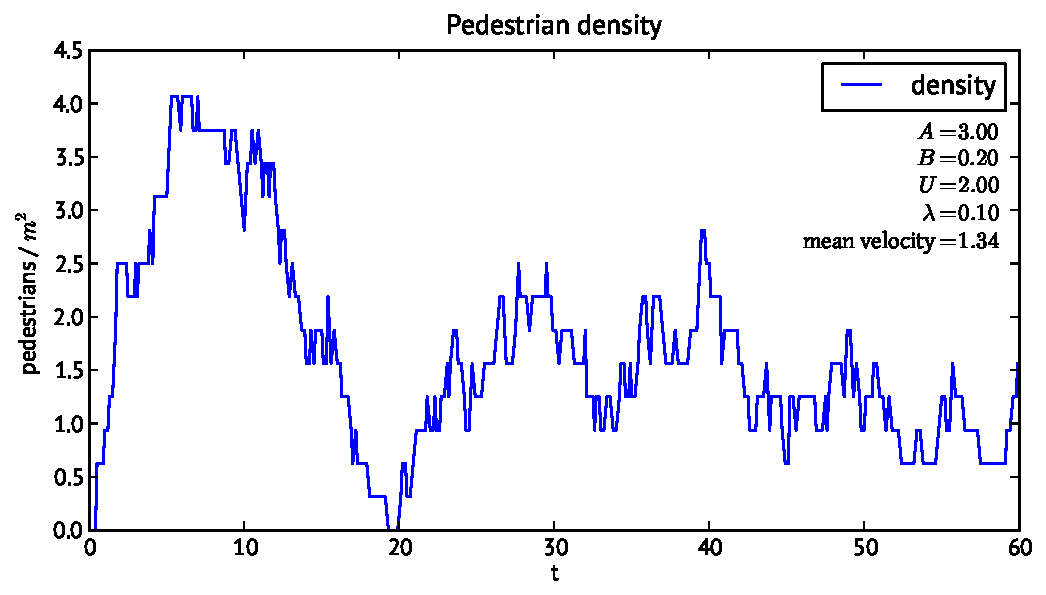
\includegraphics[scale=0.45]{Figures/dens_mvel4_relax1.pdf}}
\caption{These figures was made to see if the freezing by heating effect when raising the max velocity factor. As seen in the figures, the
density does not increase when the max desired velocity is increased. When raising the max desired velocity the density gets lower because
the pedestrians more easely get through the crowd.}
\label{fig:freezingbyheating1}
\end{figure}

\subsubsection{Intial conditions and relaxation time $0,5$ second}
\cite{helbing00} set the relaxation time to $0,5$. As the first corridor simulations we set the parameters as \cite{ABconstant}
and then change the relaxation time to $0,5$ as \cite{helbing00}. After the simulation with the initial conditions, we raise the
max desired velocity to see if we can replicate the freezing by heating effect.

The initial simulation has the values from \ref{Table_constants} with the exceptions:

\begin{itemize*}
    \item Relaxation time: $0,5 s$.
    \item Number of pedestrians: $50$ starting, adding $3/s$.
\end{itemize*}

The next simulation we keep the new relaxation time, but changes the max velocity factor set to $4.0$


When comparing the simulations we do not see the freezing by heating effect.
Instead we see that the pedestrians more easely escape the clogging, and the flow in each directions
gets more steady. In both simulations we observed lane formation.

\begin{figure}[h]
\centering
\subfloat[The figure show the density in corridor when the parameters are set as \cite{ABconstant} and \cite{helbing00}.]{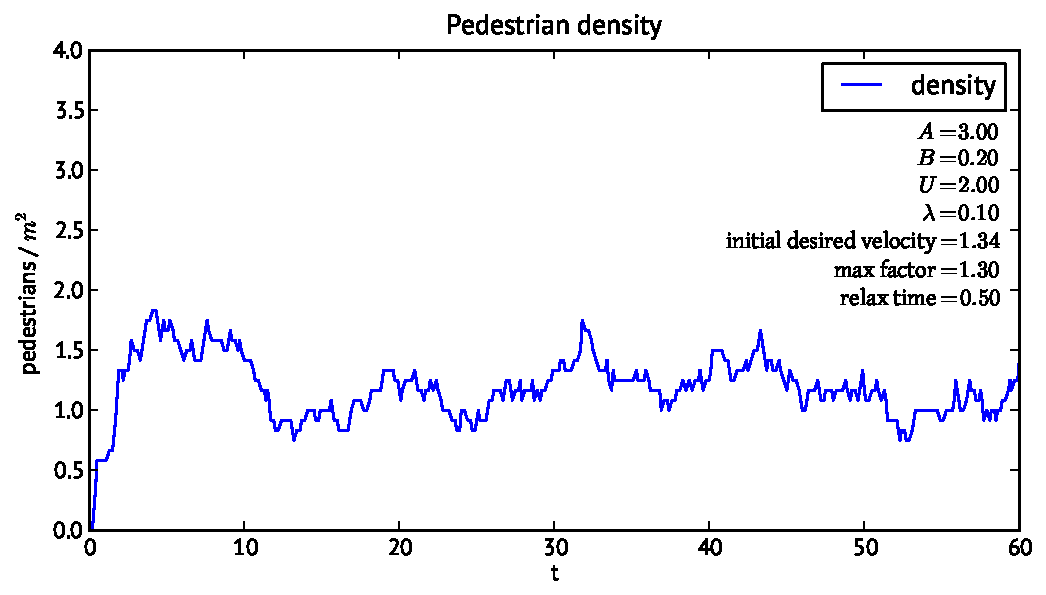
\includegraphics[scale=0.45]{Figures/dens_init_relax05.pdf}}
\subfloat[This figure shows the density in the corridor when the max velocity factor is set to $4.0$ and the max desired velocity is set to $4,0$, and the other parameters as figure a.]{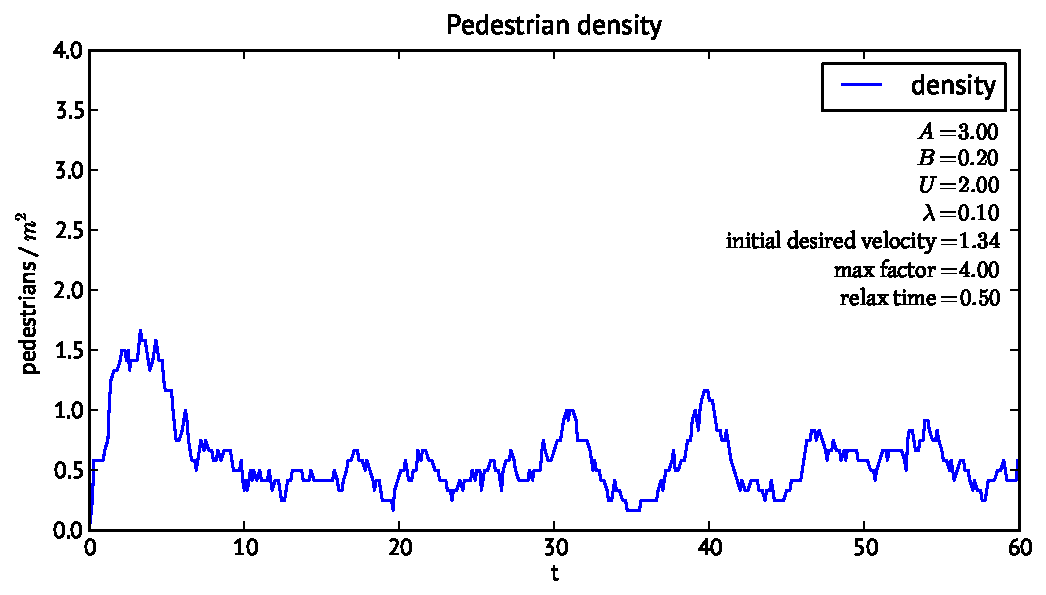
\includegraphics[scale=0.45]{Figures/dens_mvel4_relax05.pdf}}
\caption{These figures was made to see if the freezing by heating effect when raising the max velocity factor. As seen in the figures, the
density does not increase when the max desired velocity is increased. When raising the max desired velocity the density gets lower because
the pedestrians more easely get through the crowd. The difference between figure \ref{fig:freezingbyheating1} and this is the relation time,
respectively $1,0$ and $0,5$.}
\label{fig:freezingbyheating05}
\end{figure}

\subsection{The bottleneck}
In this scenario we wanted to the the oscillitory flows that is reported 
in \cite{self-org} to happen when you have a bidirectional flaw through a 
bottleneck. A print screen from the simulation is shown in figure 
\ref{fig:bottleneckbidirec}.

\begin{figure}[h]
\centering
{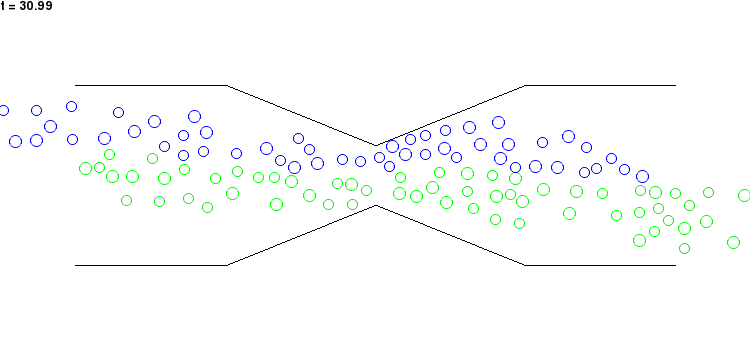
\includegraphics[scale=0.35]{Figures/bottleneck.png}}
\caption{A screen shot of the bottleneck simulation.}
\label{fig:bottleneckbidirec}
\end{figure}

\subsubsection{Attempts to see the faster is slower effect in the bottleneck}
In order to see the faster-is-slower effect we make a series of simulations 
with increasing mean velocity. The results is presented in figure 
\ref{fig:is-faster-slower-in-bottleneck}.

\begin{figure}[h]
\centering
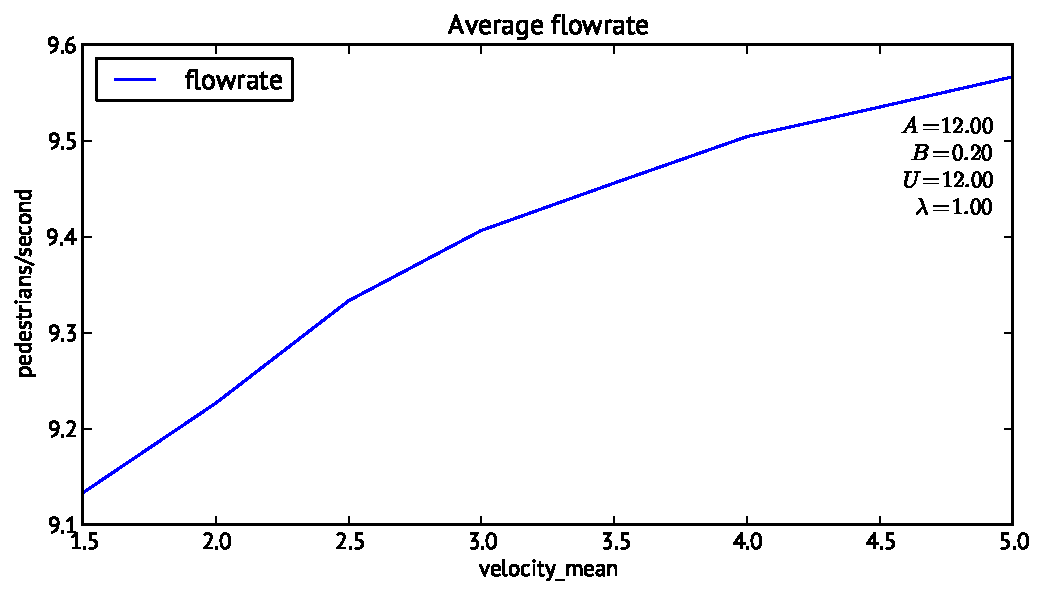
\includegraphics[scale=0.45]{Figures/Wide-kink-one-directional-flowrate-agg.pdf}
\caption{A graph of the flow rate as the average velocity is increased}
\label{fig:is-faster-slower-in-bottleneck}
\end{figure}

\subsection{The corridor with open space}
In this scenario we wanted to reproduce the results that people start to 
clock up in a corridor if there is a sudden area that allow pedestrians to try 
and overtake each other. To see if the flow rate is affected by the pedestrians 
who try to overtake each other we compare the flow rate with the wide space with 
the flow rate from a normal corridor scenario. A screen shot from each simulation 
can be seen in figure \ref{fig:widekink}.

\begin{figure}[h]
\centering
\subfloat[A screen shot of the normal corridor.]{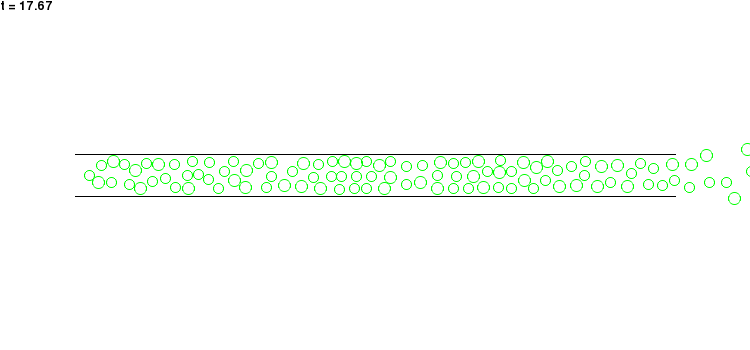
\includegraphics[scale=0.25]{Figures/normalcorridor.png}}
\subfloat[A screen shot of the corridor with a wide space.]{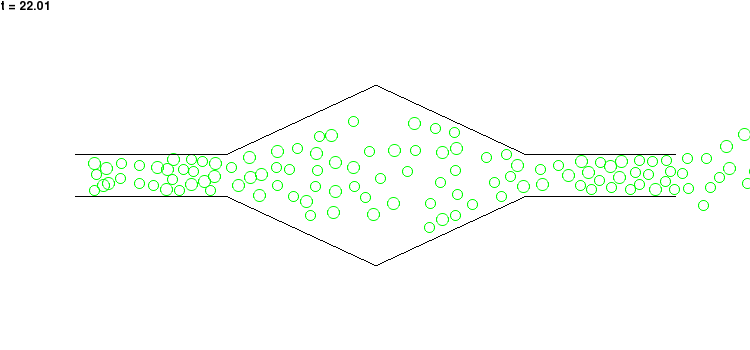
\includegraphics[scale=0.25]{Figures/Widespace.png}}
\caption{The two scenarios we want to compare to see the effect of the wide space.}
\label{fig:chokepoint}
\end{figure}

We expected to see that the flow rate in the scenario shown in figure 
\ref{fig:chokepoint} (b) would be lower than in the scenario (a). What we sat 
in shown in figure \ref{fig:effect-of-widespace}

\begin{figure}[h]
\centering
\subfloat[A graph of the mean velocity of the pedestrians in normal corridor]{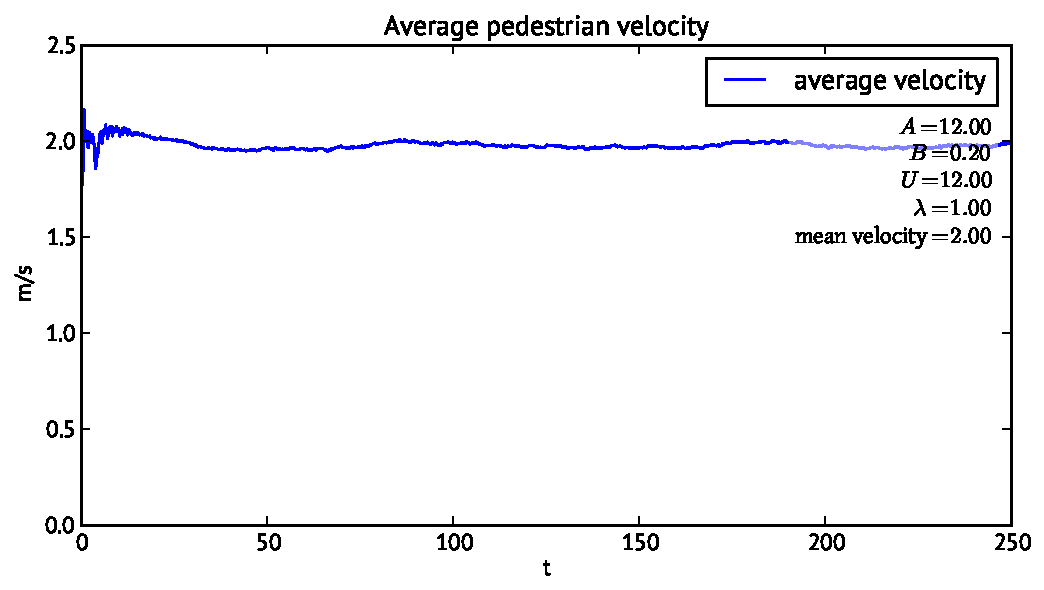
\includegraphics[scale=0.45]{Figures/corridor-velocity.pdf}}
\subfloat[A graph of the mean velocity of the pedestrian in the corridor with a wide space]{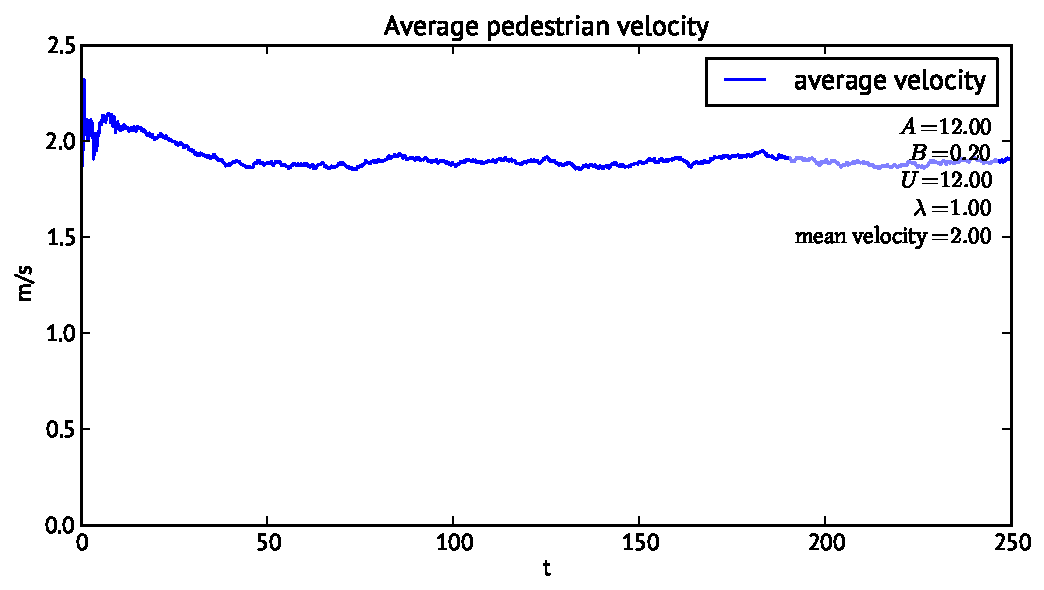
\includegraphics[scale=0.45]{Figures/bottleneck-velocity.pdf}}\\
\subfloat[A graph of the flow rate of the pedestrians in the normal corridor]{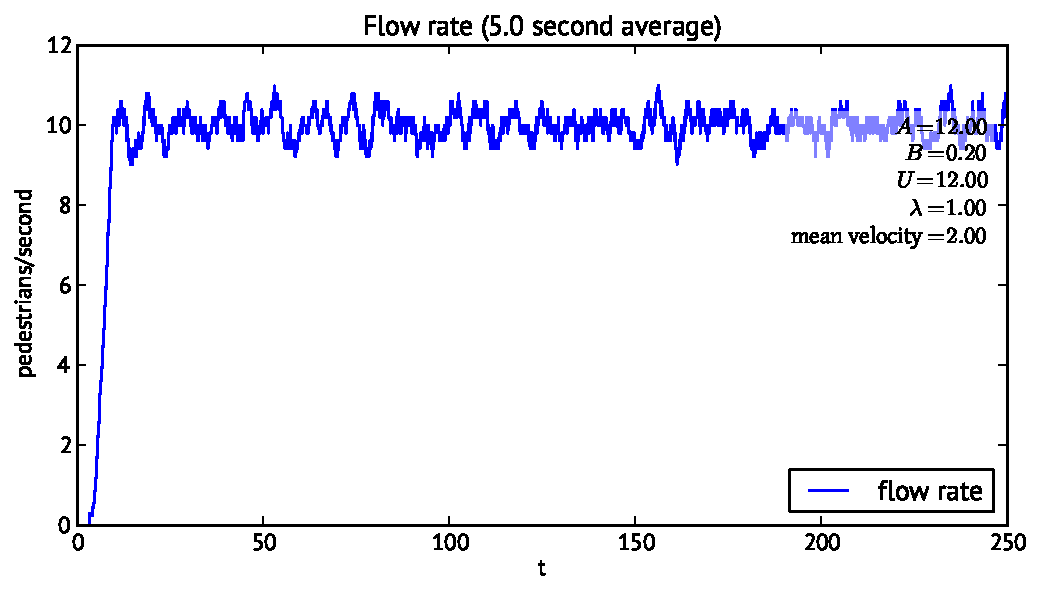
\includegraphics[scale=0.45]{Figures/corridor-flowrate.pdf}}
\subfloat[A graph of the flowrate in the corridor with the wide space]{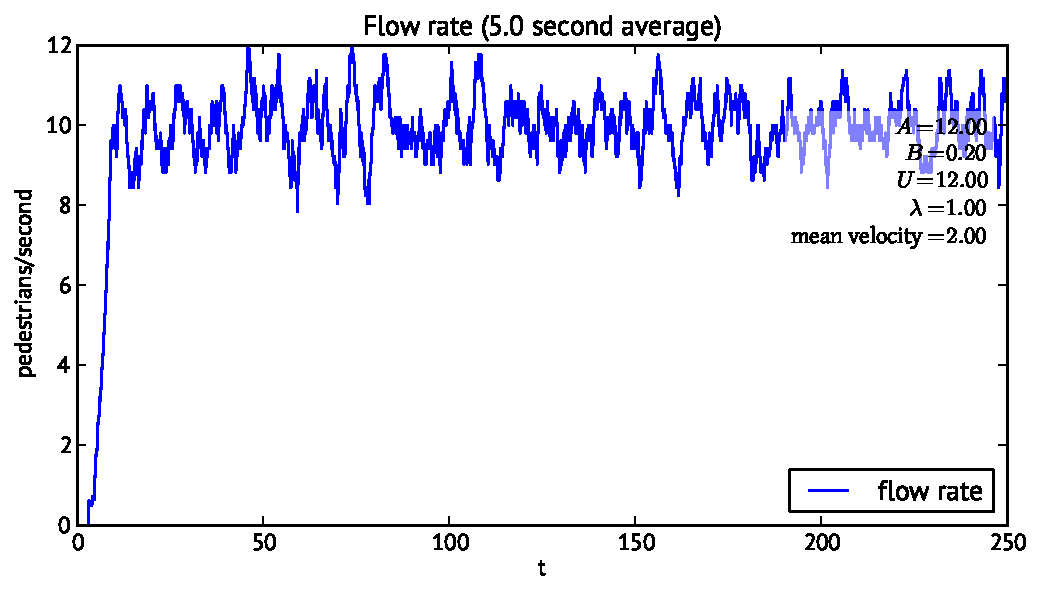
\includegraphics[scale=0.45]{Figures/bottleneck-flowrate.pdf}}
\caption{There is a lowering of the average velocity of the pedestrians due to the bottleneck. We see that there is no consistent lowering of the flowrate due to the bottleneck. What we see is that the flowrate is varying more over time.}
\label{fig:effect-of-widespace}
\end{figure}

\subsubsection{Attempts to see the faster is slower effect in the corridor with wide space}
The faster is slower effect in not observed in the extent that we would expect from 
the article. However the flow rate does not increase linearly with average velocity. 
 
\begin{figure}[h]
\centering
\subfloat[A graph of the flow rate as the average velocity is increased in the case of one directional pedestrian flow.]{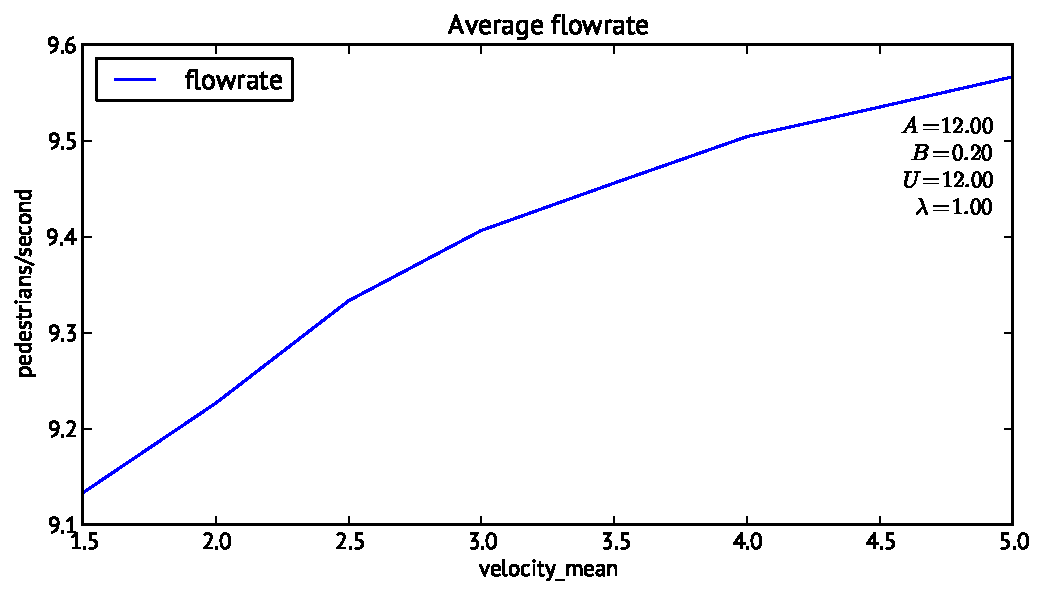
\includegraphics[scale=0.45]{Figures/Wide-kink-one-directional-flowrate-agg.pdf}}
\subfloat[A graph of the flow rate as the average velocity is increased in the case of bidirectional pedestrian flow.]{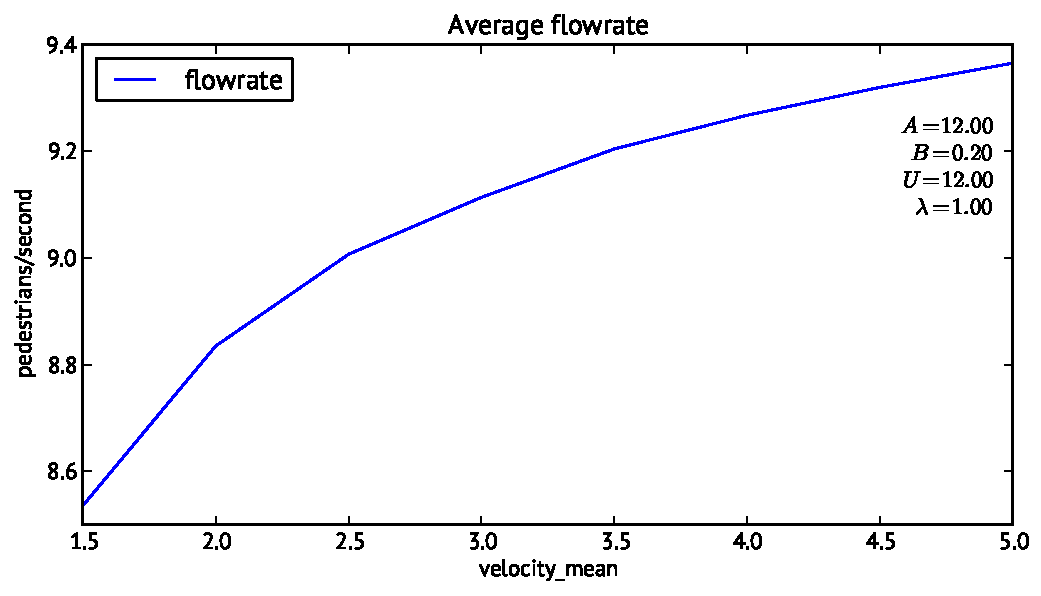
\includegraphics[scale=0.45]{Figures/Widekink-twodirectional-flowrate-agg.pdf}}
\caption{The two scenarios we want to compare to see the effect of the wide space.}
\label{fig:is-faster-slower-in-widekink}
\end{figure}

% TODO: Add parameters that are varied.

\clearpage
\section{Discussion of our results}
\label{sec:discrepancies}
As we have seen in section~\ref{sec:results}, we have not obtained the 
expected results from our simulations in all cases. In this section we discuss 
possible reasons for this discrepancy between the expected and actual results, 
and some possible changes that we believe will fix these discrepancies.

The section is divided into two parts: in the first we discuss possible errors 
related to our implementation of the simulation, and in the second part we 
discuss changes to the model that might fix some of the discrepancies.

\subsection{Our implementation of the simulations}
\label{sec:random-errors}
We have attempted to implement the simulation of the model that is as close to 
the description of the model as possible. However, as we have seen in 
section~\ref{sec:model-to-simulation}, there has been some areas where we have 
had to fill in some details that have not been explained in the articles 
describing the model. Indeed, in the formulation of the model itself, we have 
been forced to add features from different articles because the description in 
the original article was insufficient. It is possible that some of these 
necessary additions have been done differently than seen in the simulations 
performed by the authors of the original articles, and that this contributes 
to the discrepancies between the their results and ours.

Of course we cannot completely rule out errors in our implementation either; 
while we do not believe any obvious errors exist, we do not have anything to 
compare it with that has the same level of detail. The only thing we have to 
compare our implementation with, is the code underlying \cite{helbing00}, 
which the authors have published on their website. However, this code is quite 
inscrutable, so it would require considerable effort to analyse it and compare 
it with our own. A cursory glance indicates that there are features in it that 
we do not have in our implementation; whether these are vital or not we cannot 
say.

A final thing that relates to the implementation of the simulation is the 
setting of parameters and initial conditions. The values for the different 
parameters have not always been given along with their description in the 
articles describing the model. This means we have had to find the values 
elsewhere, and this mixing of parameters from different sources might also be 
a source of errors. Finally, the use of random values for initial conditions 
(in the setting of pedestrian starting positions, size and initial desired 
speed) is a possible source of error. While we set a mean value and a standard 
deviation on the generated values, in some cases extremely high or low values 
are generated. An example of this is seen in figure~\ref{fig:random-seed}, 
where one pedestrian starts out with a very low desired velocity, causing it 
to move extremely slowly. The long leaving time is then not caused by clogging 
of the exit, but simply by the delay from the time it takes the pedestrian to 
cross the distance between its starting point and the exit.

\begin{figure}[h]
    \centering
    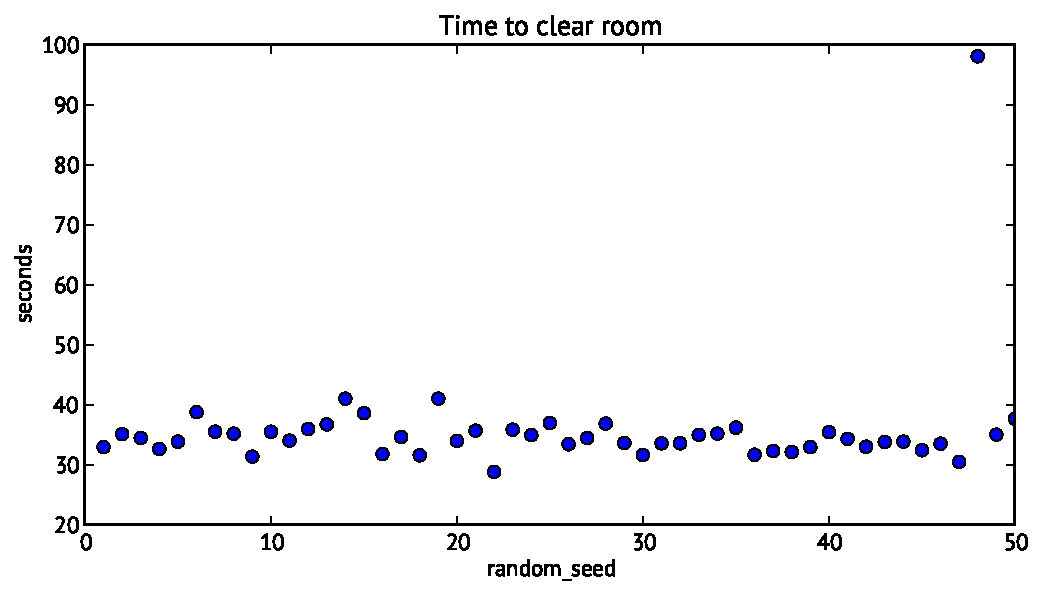
\includegraphics[width=0.8\textwidth]{Figures/random-seed-variations.pdf}
    \caption[Leaving time for different random seeds]{Leaving time for 
    different random seeds. Results are dependent on random numbers; for a 
    seed value of 48 (top-right corner), one pedestrian starts out walking 
    very slowly impacting the total leaving time.}
    \label{fig:random-seed}
\end{figure}



\subsection{Clogging in narrow places}
The article \cite{self-org} claims that social force models are able to reproduce the clogging phenomena which arises when a large number of pedestrians try to pass a narrow passage. This phenomena is also know as the "faster is slower phenomena". Through our simulation this phenomena has not occurred.



\subsection{Pedestrians overlapping and walking through walls}
A problem we encountered during the simulation was pedestrians walking through walls and/or pedestrians overlapping. Both these scenarios are illustrated in figure \ref{fig:problemSenario}. This could be caused by the size of the time step see section \ref{constants}, but the time step can not always correct this problem.

A person can have a resulting force which points towards the wall even as the distance to the wall approaches zero. This problem arise when pedestrians are moving fast and are unable to stop in time and occurs because the model do not take into account how fast pedestrians are approaching walls or other pedestrians.

In other words, a pedestrian running towards a wall will decelerate at the same rate as a person walking towards the wall. One could argue that this is unrealistic behaviour because, the person running should start decelerating sooner than the person walking. A person which has a force towards the wall which exceed the force he feels from the wall, then he will always go through the wall. This phenomena is off course not dependent on the time step, since even with a infinity small time step this could occur. One way of elimination this problem is by making the force a pedestrian feel depend not only on the distance to the obstacle but also depend on the current speed towards this obstacle. Such a feature has been documented to improve the predictions of the model\cite{ABconstant}.
\begin{figure}
\centering
\subfloat[Overlapping occurs when speeds get to high in this case $2.50m/s$ which prevents pedestrians from stopping in time.]{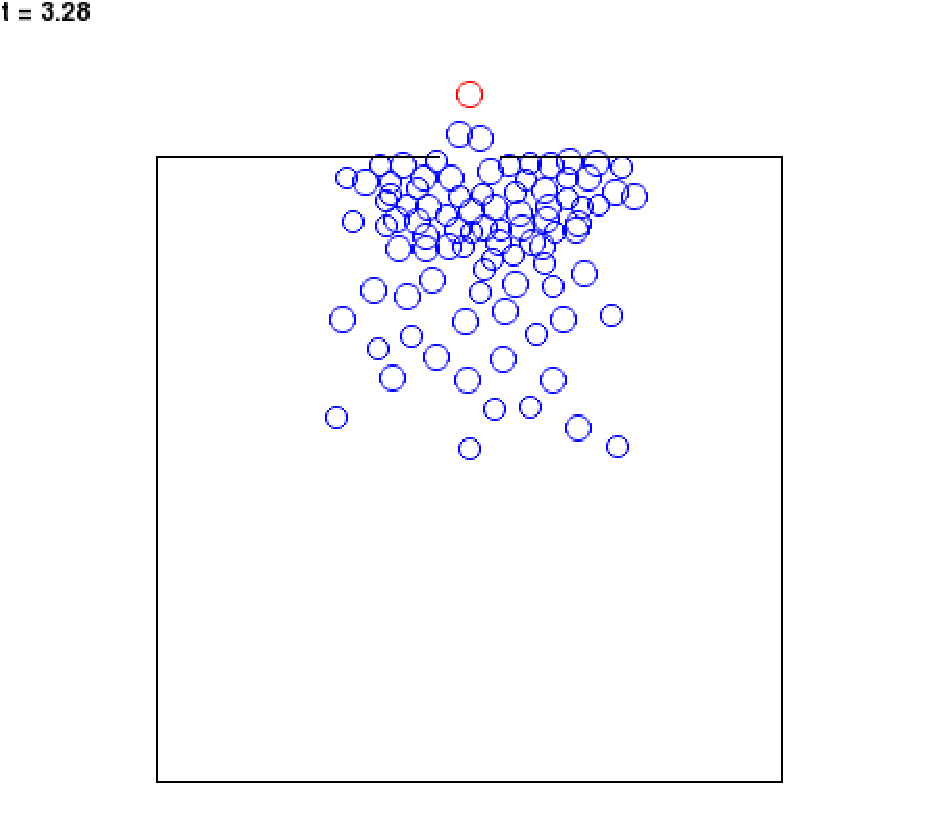
\includegraphics[scale=0.5]{Figures/squareRoomOverlapping}}
\subfloat[A single pedestrian escapes through the wall due to a initial speed of $3.50m/s$]{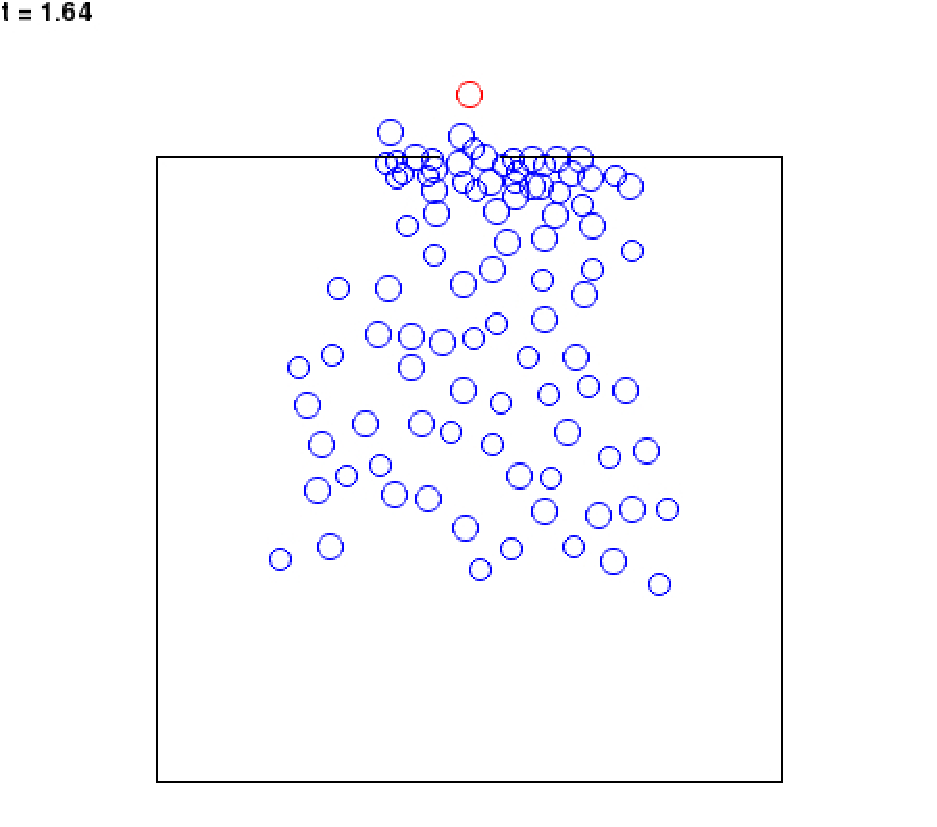
\includegraphics[scale=0.5]{Figures/squareRoomThrowWall}}
\caption{These pictures was produced with the following values: $A=2.2$, $B=0.2$, $U=2.0$, Pedestrian number=$100$, $\lambda=0.1$, $v^{max}_0=1.3 \cdot v_0$, $\tau = 1.0$, $\triangle t = 0.01$, only the starting velocity was changed}
\label{fig:problemSenario}
\end{figure}
\subsection{Faster-is-slower effect}
The article \cite{self-org} claims that social force models are models which are capable of representing the faster-is-slower effect. In our simulations people leave the room faster and faster as we increase their max speed. The article 

\subsection{Tangential forces}
Here we discuss the idea of improving the model by improving tangential forces, that is, the force parallel to the surface of an object.
The tangential forces can be used as collision avoidance, so that pedestrians steer around obstacles or other pedestrians \cite{tang}.
This would be relevant when simulating an environment where, e. g., and is standing in the middle of a symmetrical room and the pedestrian's waypoint
is behind a big square pillar, with equal distance either way around, the pedestrian would get stuck in front of the pillar without the tangential forces,
since the forces acting on the pedestrian's motivation is cancelling each other out. 
In our case where two groups of pedestrians are crossing each other in a corridor, the tangential force would make the pedestrians to into account
the position of the pedestrians in front of them and steer around them.
The tangential forces can also improve the model so it can simulate pedestrians escaping a smoke filled room where we determine the visibility.
In this case of simulation the pedestrians would walk randomly around untill they find a wall, and follow the wall around due to the tangential force.
This would be a way of implementing way finding to the model.

Friction between pedestrians would also be possible to add to the model, since the tangential forces from other pedestrians would make it
harder for pedestrians to walk through a crowd. \cite{self-org} mention that friction is causing clogging in front of exits, since the people
get stuck in each other. In our simulation the pedestrians are not clogging as heavily as \cite{self-org} mention it can be.
The time it take for the pedestrian to leave a room in unrealistic low, and we think that implementing the friction by tangential forces
would make the simulation time more realistic.

\subsection{Freezing by heating effect}
According to \cite{self-org} the freezing by heating effect should arise when the max desired velocity of the pedestrians was raised.
That is that clogging should arise when raising the max velocity of the pedestrians, because more are ariving to the possible
clogging area, and thus have more trouble getting through the crowd. 
We tried to raise the max velocity, see figure \ref{fig:freezingbyheating1} and figure \ref{fig:freezingbyheating05}, but instead of observing the freezing by heating effect, we saw that the pedestrians
got through the corridor more easely, and that the density in the corridor was lower when the max velocity was high.
We think that there are more explations to this result. For the first the pedestrian $\alpha$'s force toward the target
is higher when $\alpha$'s velocity gets higher, and therefore he more easely pushes his way through the crowd. For the second
there are no friction between the pedestrians to slow $\alpha$ speed down, besides the social sphere.

\subsection{Comparison between the relaxation time $1,0$ second and $0,5$ second}
When simulating the corridor with the initial conditions and changing the relaxation time from $1,0 s$ to $0,5 s$,
the pedestrians do not get stuck as easely when the relaxtion time is $0,5 s$ as they do when the relaxation time
is $1,0 s$. This can be seen in figure \ref{fig:comparison_of_timestep}, that in (a), the density get high faster,
while in (b) the density does not increase as fast as (a).
When the relaxation time is $0,5 s$, the pedestrians reacts faster, in the sense that they speed up faster,
after collisions with pedestrians walking in the other direction.

\begin{figure}[h]
\centering
\subfloat[The figure show the density in corridor when the relaxation time is set to $1,0 s$]{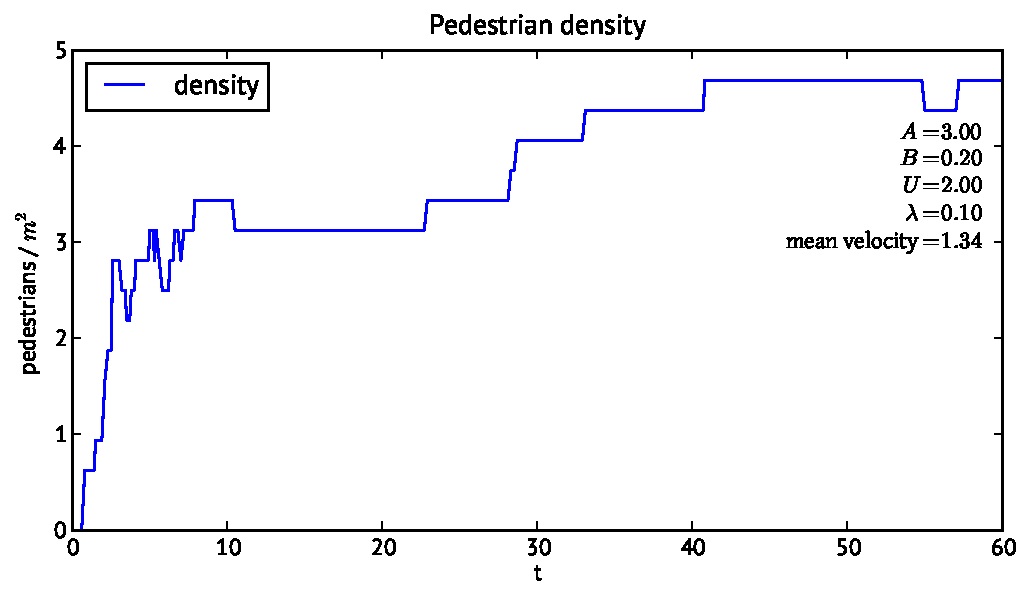
\includegraphics[scale=0.45]{Figures/dens_init_relax1.pdf}}
\subfloat[This figure shows the density in the corridor when the relaxation time is set to $0,5 s$]{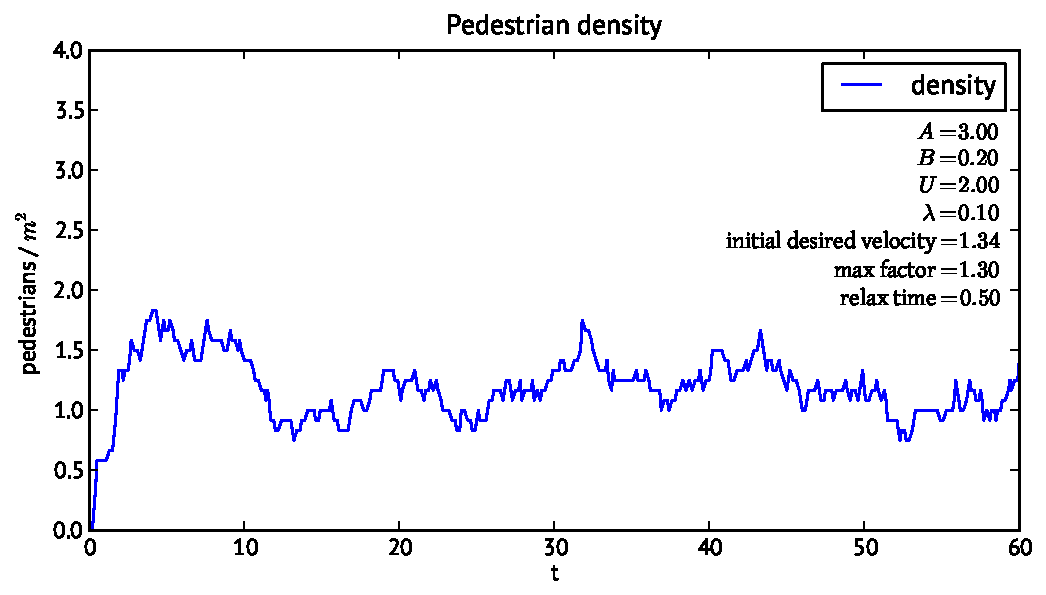
\includegraphics[scale=0.45]{Figures/dens_init_relax05.pdf}}
\caption{These figures show the difference of the density when changing the relaxation time of the model from $1,0 s$ to $0,5 s$.
It is seen the the density is more steady when the relaxtion time is $0,5 s$ instead of $1,0 s$}
\label{fig:comparison_of_timestep}
\end{figure}

A possible explanation of why the density is more steady through out the simulation when the relaxation time is $0,5 s$,
is that the pedestrians reacts faster to changes of their velocity. Thus when they bump into each other, they speed up
faster, and therefore avoid clogging up before more get in their path.


\clearpage
\section{Assessment of social force models}
\label{sec:assessment}
In this section we will present our assessment of social force models in 
general, based on our work with the specific model and the results we have 
obtained. Based on our results, we will outline the advantages and weaknesses 
of social force models in general, and conclude by assessing the state of 
these types of models.

\subsection{Advantages of social force models}
The main advantage of using social force models for modelling crowds is 
expressed quite well in this quote from \cite{self-org}:

\begin{quote}
    The advantage of the social force-based simulation approach is its simple 
    form and its small number of parameters, which do not need to be 
    calibrated anew for each situation.
\end{quote}

That is, using this approach allows us to simulate a complex system using a 
quite simple formulation of the model. Simulating a large crowd of pedestrians 
using a classical (i.e. non-agent based) model would be very complex, and 
quite possibly impractical.

This simplification is possible, because the complexities of the model 
behaviour is moved from the formulation of the model and into the 
calculations. That is, a very large number of calculations are needed to get 
any meaningful results out of this model. This means that working with this 
kind of model would be impractical without the help of computers, and indeed a 
large quantity of processing power is necessary to get any results. In our 
simulations this has been most apparent in the need to implement the 
calculation-intensive parts of the model in the C programming language, to be 
able to achieve reasonable computation times.

Another advantage of the simulations we get from the model, is that it is very 
straight forward to inspect the results visually, because it is possible to 
create drawings of the simulation steps. This means that comparing the 
simulations to e.g. videos of real-life crowds, and spotting effects such as 
the lane formation becomes trivial. It is also an advantage that simulations 
can be run in real time, so making visual assessments of results is easy.

Of course having a simple model that is practical to implement is of no use if 
it does not give useful results. Empirical studies have shown that social 
force models are able to show phenomena that correspond to real crowds, and as 
such do provide meaningful results in some cases. However, while parameters 
may not need to be calibrated for each situation, as the quote above says, 
calibration is required, and doing so is non-trivial. This means that we have 
not been able to identify parameters for our simulations that work across all 
the different scenarios.

\subsection{Weaknesses of social force models}
While social force models in some cases have been shown to give results that 
correspond to real life observations, there are several weaknesses to this 
approach to modelling crowds. Some of these weaknesses are related to the way 
the models are presented, and some are more fundamental to the nature of 
social force models.

When working with social force models, we have had to piece together a working 
model from several different sources. This exposes a difficulty in assessing 
the models: It is not always obvious if a given weakness is due to an inherent 
quality of the models, or if it is simply due to a weak or missing formulation 
of some part of it. Especially precise results of simulations have been 
difficult to find, and as has been shown in 
section~\ref{sec:model-to-simulation}, we have had to fill in several details 
ourselves. As mentioned above, the difficulty in estimating parameters has 
also provided a barrier in this respect.

Setting aside the difficulties in finding detailed information about the 
model, it is readily apparent that social force models are in a relatively 
early state of development. This means that the amount of empirical data 
available to assess the quality of the models' predictions is quite low. This 
means that even if the social force models have shown some promising results, 
it is impossible to say with confidence that they do indeed predict the actual 
behaviour of crowds very well.

Further compounding these uncertainties is the fact that the model is 
formulated in a way that is counter-intuitive to the way human behaviour is 
normally perceived. That human behaviour is reducible to simple repulsive 
forces is counter to what we believe is reasonable to expect. This means that 
if this is indeed the case, strong evidence is needed to convince us, which is 
not currently provided.

One of the reasons we are sceptic that these forces are able to completely 
explain human behaviour, is that they pertain to behaviour of objects in a 
physical world, but they do not obey the traditional physical laws of motion.  
It is clear that the idea of using forces to describe movement has its origins 
in physics, but excluding some of the properties of physical forces seems 
arbitrary.

Finally, the fact that different variants of social force models use 
completely different parameters and formulations of the different forces, 
sometimes even contradicting each other, makes it seem as though the models 
are changed in arbitrary ways to accommodate empirical observations. This 
belief is corroborated by the fact that the models do not make any new 
predictions that are then tested, but instead only seem to attempt to 
replicate already observed behaviour.

\subsection{Conclusion on the assessment}
Weighing the advantages and disadvantages of social force models against each 
other, it is quite apparent that the models do not instil a strong sense of 
confidence in their predictions. However, the crucial advantage that these 
models have, is that they are able to do \emph{some} predictions of crowd 
behaviour, that no other models have been able to. This means that while 
social force models are far from perfect, they are in many ways the best 
available way of evaluating e.g. a new building's suitability for efficient 
crowd movement. And while the models may not be able to provide any underlying 
mechanisms or reasons for crowd behaviour, in practice they may, given further 
adjustments and experiments with real life observations, be a substantial 
improvement over today's standards.

\clearpage
% vim:ft=tex
\section{Conclusion}
\label{sec:conclusion}

\subsection{Further work}
Since the simulation we present in the report has not shown some properties of 
a crowd, if given more time our group would like try to solve the 
discrepancies and add the possible solutions that has been talked about in 
section \ref{sec:discussion}. The first thing to do maybe modify the repulsive 
forces and add the frictional force, and make them velocity dependent, which 
will make the crowd behave more realistic.  To enable the model to simulate 
more complex situation, we will need the path finding feature. Also a set of 
parameters should be determined when the environment is changed, and the 
method to attain those parameters may be the same as what the Helbing group 
has been doing, that is by doing some experiments and analysing the video 
track.

\clearpage
\bibliographystyle{ruc}
\bibliography{crowd-modelling}
\clearpage

\end{document}
